%% ═══════════════════════════════════════════════════════════════════════════
%% APPENDIX — included via %% ═══════════════════════════════════════════════════════════════════════════
%% APPENDIX — included via %% ═══════════════════════════════════════════════════════════════════════════
%% APPENDIX — included via %% ═══════════════════════════════════════════════════════════════════════════
%% APPENDIX — included via \input{appendix} from main.tex
%% ═══════════════════════════════════════════════════════════════════════════

\section{Data Summary}\label{app:data_summary}

A comprehensive overview of all data variables used in this thesis, their sources, and their roles in the analysis is provided in Table~\ref{tab:data_summary}.

\begin{table}[H]
\centering
\small
\begin{tabular}{l l l l}
\toprule
Variable & Source & Description & Used in \\
\midrule
\multicolumn{4}{l}{\emph{Stock-level variables}} \\
Monthly returns & CRSP \texttt{msf} & Adjusted holding-period returns & Sections 3, 5 \\
Price, shares out. & CRSP \texttt{msf} & For market equity computation & Section 3.5 \\
Exchange, share codes & CRSP \texttt{msf} & Universe filtering (codes 10, 11) & Section 3.2 \\
Delisting returns & CRSP \texttt{msedelist} & Survivorship bias correction & Section 3.2 \\
Book equity (\texttt{ceqq}) & Compustat \texttt{fundq} & Book-to-market, ROE & Section 3.5 \\
Total assets (\texttt{atq}) & Compustat \texttt{fundq} & Asset growth, gross profit & Section 3.5 \\
Income (\texttt{ibq}) & Compustat \texttt{fundq} & ROE, earnings growth & Section 3.5 \\
Revenue (\texttt{revtq}) & Compustat \texttt{fundq} & Gross profitability & Section 3.5 \\
COGS (\texttt{cogsq}) & Compustat \texttt{fundq} & Gross profitability & Section 3.5 \\
Debt (\texttt{dlttq}, \texttt{dlcq}) & Compustat \texttt{fundq} & Leverage ratio & Section 3.5 \\
\midrule
\multicolumn{4}{l}{\emph{Market-level variables (HMM inputs)}} \\
Daily market returns & CRSP \texttt{dsi} & Realised volatility (VOL) & Section 3.3 \\
Market price index & CRSP \texttt{dsi} & Drawdown (DD) & Section 3.3 \\
Cross-sect.\ stock returns & CRSP \texttt{msf} & Dispersion (DISP), REL\_N & Section 3.3 \\
\midrule
\multicolumn{4}{l}{\emph{Derived features}} \\
$mom_1, \dots, mom_{12}$ & Computed & 12 trailing momentum signals & Section 3.5 \\
$\pi_t^{\text{filter}}$ & HMM output & Filtered panic probability & Section 4.1 \\
7 fundamentals & Computed & bm, roe, gross profit, etc. & Section 3.5 \\
\bottomrule
\end{tabular}
\caption{Summary of all data variables used in the analysis.}
\label{tab:data_summary}

\medskip
\small
\textbf{Notes:} All data accessed via WRDS. Compustat linked to CRSP via the CCM bridge table using primary link types (LU, LC). Fundamentals are lagged four months from fiscal quarter end to ensure real-time availability. The sample covers January 1990 to November 2025 (training: 1990--2010; test: 2011--2025).
\end{table}

\section{Portfolio Formation, Transaction Costs, and Performance Metrics}\label{app:portfolio}

\subsection{Portfolio Construction}\label{app:portfolio_construction}

For each method, a long-only top-decile portfolio is constructed each month. A long-only construction is chosen because it consistently outperformed long-short alternatives in preliminary tests, a finding consistent with the strong upward market trend over the 2011--2025 test period, which penalises short positions. Stocks are ranked by their scores, and NYSE-listed stocks are used to determine the 90th percentile breakpoint. All stocks (including AMEX and NASDAQ) whose score exceeds this threshold enter the long portfolio.

Portfolio weights are assigned proportionally to market equity (value-weighting):
\begin{equation}
    w_t^s = \frac{ME_t^s}{\sum_{s \in \mathcal{L}_t} ME_t^s}, \qquad s \in \mathcal{L}_t,
\end{equation}
where $\mathcal{L}_t$ is the set of stocks in the long portfolio at month $t$. Value-weighting tilts the portfolio toward large, liquid stocks, reducing the influence of small-cap return anomalies and improving implementability.

\subsection{Rebalancing Frequency}\label{app:rebalancing}

Two rebalancing schemes are evaluated. Under monthly rebalancing, the portfolio is reconstituted every month using updated scores. Under quarterly rebalancing, stocks are re-scored and traded only in March, June, September, and December; in intervening months, holdings are carried forward and weights drift with market capitalization changes. No transaction costs are incurred during hold months.

\subsection{Transaction Costs}\label{app:transaction_costs}

A one-way transaction cost of $c = 10$ basis points is applied at each rebalancing date. The net portfolio return at rebalancing month $t$ is:
\begin{equation}
    r_t^{\text{net}} = r_t^{\text{gross}} - c \cdot \tau_t,
\end{equation}
where $\tau_t$ is the one-way portfolio turnover:
\begin{equation}
    \tau_t = \frac{1}{2} \sum_{s} \left|w_{t}^{s,\text{new}} - w_{t-1}^{s,\text{prev}}\right|,
\end{equation}
and the summation runs over all stocks appearing in either the new or previous portfolio. The 10 basis point cost reflects the transaction environment for a value-weighted, large-cap-biased strategy where NYSE breakpoints tilt toward liquid securities.

It is important to note that transaction costs are applied \emph{post-hoc} as an accounting adjustment and are not incorporated into the models' training objectives. The cross-sectional models (Methods~0--2) optimise stock-level prediction (classification accuracy or return forecasting) without knowledge of the previous portfolio, the resulting turnover, or the cost of rebalancing. This is standard practice in the empirical asset pricing literature \citep[e.g.,][]{FamaFrench2015, GHM2023}, where portfolio construction is treated as a fixed downstream step applied uniformly to all strategies. An end-to-end framework that jointly optimises stock selection and portfolio-level objectives (e.g., net-of-cost Sharpe ratio) would require a fundamentally different architecture, such as a reinforcement learning or differentiable portfolio optimisation layer, and remains a potential extension of this work.

\subsection{Performance Metrics}\label{app:evaluation}

\paragraph{Standard Metrics}\label{app:standard_metrics}

Strategy performance is assessed using four standard risk-adjusted metrics computed on monthly net-of-fee returns.

\textbf{Annualized return} The geometric annualized return over $n$ months is:
\begin{equation}
    R_{\text{ann}} = \left[\prod_{t=1}^{n}(1 + r_t)\right]^{12/n} - 1.
\end{equation}

\textbf{Annualized volatility} The annualized standard deviation of monthly returns:
\begin{equation}
    \sigma_{\text{ann}} = \sigma(r) \cdot \sqrt{12}.
\end{equation}

\textbf{Sharpe ratio} The annualized Sharpe ratio:\footnote{All Sharpe ratios in this thesis are computed using raw returns rather than excess returns above the risk-free rate. Since the same convention is applied to every strategy, relative comparisons and rankings are unaffected. The risk-free rate was near zero for most of the test period (2011--2021) and averaged roughly 2\% annualized over the full 2011--2025 window, so absolute Sharpe ratios are overstated by approximately 0.05--0.10.}
\begin{equation}
    SR = \frac{\bar{r}}{\sigma(r)} \cdot \sqrt{12},
\end{equation}
where $\bar{r}$ is the mean monthly return.

\textbf{Maximum drawdown} Let $C_t = \prod_{\tau=1}^{t}(1 + r_\tau)$ denote the cumulative wealth path. The maximum drawdown is:
\begin{equation}
    MDD = \min_{1 \leq t \leq n} \frac{C_t - \max_{1 \leq \tau \leq t} C_\tau}{\max_{1 \leq \tau \leq t} C_\tau}.
\end{equation}

\paragraph{Regime-Conditional Evaluation}\label{app:regime_eval}

To assess whether the regime signal adds value beyond unconditional stock selection, performance is decomposed by market regime. Months are partitioned into calm ($\pi_t^{\text{filter}} < 0.5$) and panic ($\pi_t^{\text{filter}} \geq 0.5$) periods, and the Sharpe ratio is computed separately within each subset:
\begin{equation}
    SR_{\text{calm}} = \frac{\bar{r}_{\text{calm}}}{\sigma(r_{\text{calm}})} \cdot \sqrt{12}, \qquad SR_{\text{panic}} = \frac{\bar{r}_{\text{panic}}}{\sigma(r_{\text{panic}})} \cdot \sqrt{12}.
\end{equation}
This decomposition helps assess whether the strategy's alpha originates primarily from calm-period stock selection, panic-period risk avoidance, or both.

\section{Feature Importance Methods}\label{app:feature_importance}

\subsection{SHAP Values for XGBoost}\label{app:shap}

To interpret the XGBoost model and assess the marginal contribution of each feature, SHAP \citep[SHapley Additive exPlanations;][]{Lundberg2017} values are computed on the test set. The SHAP value of feature $j$ for observation $\mathbf{x}$ measures its average marginal contribution to the prediction across all possible feature orderings:
\begin{equation}
    \phi_j(\mathbf{x}) = \sum_{S \subseteq N \setminus \{j\}} \frac{|S|!\,(p - |S| - 1)!}{p!} \Big[f_{S \cup \{j\}}(\mathbf{x}) - f_S(\mathbf{x})\Big],
\end{equation}
where $N$ is the full feature set, $p = |N|$, and $f_S(\mathbf{x})$ is the expected model output when only features in $S$ are observed. For tree-based models, the TreeSHAP algorithm \citep{Lundberg2020} computes these values exactly in polynomial time. The overall importance of each feature is summarised as:
\begin{equation}
    I_j = \frac{1}{n_{\text{test}}} \sum_{i=1}^{n_{\text{test}}} |\phi_j(\mathbf{x}_i)|.
\end{equation}

Two additional analyses are performed. First, the mean absolute SHAP value of $\pi_t^{\text{filter}}$ is computed separately for calm and panic months to assess whether the regime signal's influence varies across market states. Second, regime-specific XGBoost models are trained on calm-only and panic-only subsets of the training data, and their SHAP feature importances are compared to identify which features the model relies on differentially across regimes.

\subsection{Logistic Regression Coefficient Analysis}\label{app:lr_analysis}

For the logistic regression model (Method~1), feature importance is assessed directly through the estimated coefficient vector $\boldsymbol{\beta}$. Since all features are standardised prior to fitting, the coefficients are comparable in magnitude. The predicted log-odds of an above-median return decompose as:
\begin{equation}
    \log \frac{P(y_t^s = 1 \mid \mathbf{x}_t^s)}{1 - P(y_t^s = 1 \mid \mathbf{x}_t^s)} = \beta_0 + \sum_{j=1}^{p} \beta_j \tilde{x}_{t,j}^s,
\end{equation}
where $\tilde{x}_{t,j}^s$ is the standardised value of feature $j$. The absolute magnitude $|\beta_j|$ reflects the feature's marginal contribution to the log-odds per standard deviation change, providing a linear analogue to the nonlinear SHAP importance from XGBoost.

\section{Alternative Training Targets for XGBoost}\label{app:alt_targets}

The risk-aversion analysis in Section~\ref{sec:risk_aversion} uses the mean-variance utility target $y_t^s = r_{t+1}^s - \frac{\gamma}{2}\sigma_s^2$. To verify that the finding -- risk penalties reduce the Sharpe ratio by suppressing regime-adaptive bets -- is not an artefact of this particular functional form, Table~\ref{tab:alt_targets} reports XGBoost performance under three families of training targets with varying risk tolerance.

\begin{table}[H]
\centering
\small
\begin{tabular}{l l r r r r}
\toprule
Target family & Parameter & Sharpe & Ann.\ Ret & Ann.\ Vol & MDD \\
\midrule
Baseline ($r$) & -- & 1.007 & 21.6\% & 21.8\% & $-$26.1\% \\
\midrule
\multirow{5}{*}{Mean-variance: $r - \frac{\gamma}{2}\sigma^2$}
 & $\gamma = 0.5$ & 0.918 & 16.7\% & 18.8\% & $-$27.9\% \\
 & $\gamma = 1$   & 0.911 & 16.0\% & 18.1\% & $-$26.5\% \\
 & $\gamma = 2$   & 0.770 & 12.0\% & 16.5\% & $-$29.8\% \\
 & $\gamma = 5$   & 0.760 & 11.4\% & 16.0\% & $-$32.7\% \\
 & $\gamma = 10$  & 0.748 & 11.3\% & 16.1\% & $-$33.1\% \\
\midrule
\multirow{5}{*}{Log mean-variance: $\log(1{+}r) - \frac{\gamma}{2}\sigma^2$}
 & $\gamma = 0.5$ & 0.842 & 13.2\% & 16.4\% & $-$27.5\% \\
 & $\gamma = 1$   & 0.859 & 13.3\% & 16.1\% & $-$28.2\% \\
 & $\gamma = 2$   & 0.712 & 10.4\% & 15.7\% & $-$31.5\% \\
 & $\gamma = 5$   & 0.725 & 10.7\% & 15.9\% & $-$32.9\% \\
 & $\gamma = 10$  & 0.689 & 10.2\% & 16.1\% & $-$33.8\% \\
\midrule
\multirow{4}{*}{Sharpe-like: $r\,/\,\sigma^a$}
 & $a = 0.5$ & 0.920 & 16.7\% & 18.8\% & $-$28.3\% \\
 & $a = 1.0$ & 0.803 & 13.2\% & 17.5\% & $-$32.7\% \\
 & $a = 1.5$ & 0.914 & 13.7\% & 15.4\% & $-$31.0\% \\
 & $a = 2.0$ & 0.894 & 11.8\% & 13.6\% & $-$26.5\% \\
\bottomrule
\end{tabular}
\caption{Out-of-sample performance of XGBoost (M2) under alternative training targets. All models use the same features, hyperparameters, and portfolio construction. The baseline (raw return) achieves the highest Sharpe ratio; every risk-adjusted target reduces returns faster than volatility. The result is robust across all three functional forms and all parameter values tested.}
\label{tab:alt_targets}
\end{table}

The pattern is consistent: returns fall faster than volatility under every risk penalty, regardless of functional form. The mildest adjustments (mean-variance with $\gamma = 0.5$, Sharpe-like with $a = 0.5$) come closest to the baseline but still underperform. This confirms that the finding in Section~\ref{sec:risk_aversion} is not specific to the mean-variance utility formulation.

\section{Robustness Checks}\label{app:robustness}

This section reports five robustness checks that complement the main results in Section~\ref{sec:results}.

\subsection{Sub-Period Stability}\label{app:subperiod}

To assess whether the main findings are driven by a single favourable sub-period, the test sample is split into three roughly equal windows: 2011--2015, 2016--2020, and 2021--2025.

\input{tables/table_subperiod}

M1 is the most temporally stable strategy, maintaining a Sharpe ratio above 0.93 in every sub-period. M2 is similarly consistent (0.92--1.09). By contrast, fixed 12-month momentum collapses to 0.42 in the most recent sub-period, a window characterised by elevated inflation, rapid rate hikes, and two sharp corrections -- precisely the conditions under which an unconditional momentum strategy struggles and a regime-conditioned approach should add value.

\subsection{Turnover and Transaction Cost Sensitivity}\label{app:turnover}

A strategy's net-of-cost performance depends critically on its turnover. Table~\ref{tab:turnover} reports average monthly one-way turnover for each strategy.

\input{tables/table_turnover}

M1's low turnover (10.1\% per month) reflects the stability of its quality-momentum selections: the same large, profitable momentum winners tend to remain in the portfolio month after month. M2's higher turnover (64.2\%) arises from its regime-conditional switching between different stock types. Fixed 1-month momentum has the highest turnover (91.3\%), as the set of recent winners changes almost entirely each month.

Table~\ref{tab:cost_sensitivity} translates these turnover differences into Sharpe ratio sensitivity across a range of transaction cost assumptions.

\input{tables/table_cost_sensitivity}

M1 is nearly immune to transaction costs: even at 50\,bps one-way (five times the baseline), its Sharpe ratio declines by only 0.04. M2 degrades more noticeably but remains above 0.87 at 50\,bps. The baseline 10\,bps assumption is therefore conservative for M1 and reasonable for M2.

\subsection{XGBoost Hyperparameter Sensitivity}\label{app:xgb_sensitivity}

The XGBoost model uses hyperparameters selected via cross-validation on the training set. To verify that the results are not an artefact of a particular configuration, Table~\ref{tab:xgb_hyperparams} reports out-of-sample performance under alternative tree depths, learning rates, and ensemble sizes.

\input{tables/table_xgb_hyperparams}

The Sharpe ratio ranges from 0.93 to 1.12 across all configurations tested. The baseline (depth=4, lr=0.05, $n$=500) is not the single best configuration -- a lower learning rate (0.01) achieves a Sharpe of 1.12 -- but all variants meaningfully exceed unconditional momentum (Sharpe $\approx$ 0.70). The results are robust to reasonable hyperparameter perturbations.

\subsection{Regime Threshold Sensitivity}\label{app:threshold}

The regime-conditional analysis in Section~\ref{sec:regime_results} uses $\pi_t^{\text{filter}} = 0.50$ to classify months as calm or panic. Table~\ref{tab:threshold_sensitivity} checks whether the findings are sensitive to this cutoff.

\input{tables/table_threshold_sensitivity}

The regime-conditional Sharpe ratios are stable across all three thresholds, with panic-period Sharpes ranging from 1.45 to 1.52 for M1 and calm-period Sharpes from 0.76 to 0.80. The qualitative finding -- that panic months contribute higher Sharpe ratios than calm months -- holds regardless of the classification threshold.

\subsection{Number of Hidden States}\label{app:num_states}

The baseline HMM uses $K = 2$ states (calm and panic). A natural question is whether finer regime granularity -- for example, distinguishing mild corrections from severe crises -- would improve the downstream portfolio models. Table~\ref{tab:multistate_hmm} reports out-of-sample Sharpe ratios for $K = 2, 3, 4, 5$, each averaged over five independent Gibbs sampler seeds.

\input{tables/table_multistate_hmm}

M1 is completely insensitive to $K$, consistent with its near-zero loading on $\pi_t^{\text{filter}}$. M2 shows no consistent improvement beyond $K = 2$: the mean Sharpe ratios for $K = 3, 4, 5$ (0.90, 1.02, 1.03) are within one standard deviation of the $K = 2$ baseline (1.00), and cross-seed variability increases with $K$. The $K = 3$ model actually performs worst on average, despite one seed producing a Sharpe of 1.14 -- illustrating the danger of drawing conclusions from a single run.

The intermediate states that emerge for $K \geq 3$ are interpretable -- they typically capture periods of elevated volatility without deep drawdowns -- but they lack the persistence needed to provide a stable conditioning signal. In the $K = 3$ model, the intermediate state has a self-transition probability of only 0.83 compared to 0.94 for stressed and 0.94 for calm, meaning the model frequently reclassifies months between intermediate and the other states across seeds. With only 241 training months, the data cannot reliably separate more than two regimes for the purpose of downstream cross-sectional stock selection.

\section{External Validity}\label{app:external_validity}

\subsection{Alternative Train/Test Splits}\label{app:alt_splits}

To assess sensitivity to the choice of training period, the full pipeline (HMM estimation, feature construction, and ML model training) is re-run under four alternative train/test splits.

\input{tables/table_alt_splits}

Both M1 and M2 produce positive Sharpe ratios across all splits (0.78--1.04 for M1, 0.83--1.00 for M2). Returns are remarkably stable at 20--22\% annualised for M2; what varies is volatility, which is higher when the test period includes the 2008 crisis.

\subsection{Placebo Regime Signals}\label{app:placebo}

To rule out the possibility that XGBoost benefits from any additional feature rather than specifically from the HMM regime signal, the real $\pi_t^{\text{filter}}$ is replaced with five placebo variants: temporally shuffled versions (which preserve the marginal distribution but destroy temporal structure), pure random noise, an inverted signal ($1 - \pi_t^{\text{filter}}$), and a VIX-based alternative.

\input{tables/table_placebo}

M1 is completely invariant to the regime signal, achieving a Sharpe of approximately 1.03 regardless of input. M2 achieves its highest Sharpe (0.94) with the real HMM signal; all placebo variants produce lower performance. The inverted signal (0.92) comes closest, which is consistent with XGBoost learning to reverse the interpretation of the flipped input.

\subsection{Kitchen-Sink Test}\label{app:kitchen_sink}

A further concern is that XGBoost's improvement from adding $\pi_t^{\text{filter}}$ reflects the model's ability to extract spurious patterns from any additional feature. To test this, XGBoost is augmented with a single random walk feature (cumulative sum of standard normal draws) in place of $\pi_t^{\text{filter}}$, repeated 10 times with different seeds.

\input{tables/table_kitchen_sink}

Adding a random feature \emph{hurts} performance (mean Sharpe 0.75 vs.\ 0.85 without), while the real $\pi_t^{\text{filter}}$ improves it to 0.94. The regime signal's contribution is specific and economically meaningful, not an artefact of model flexibility.

\section{Convergence Diagnostics}\label{app:convergence}

\begin{figure}[H]
    \centering
    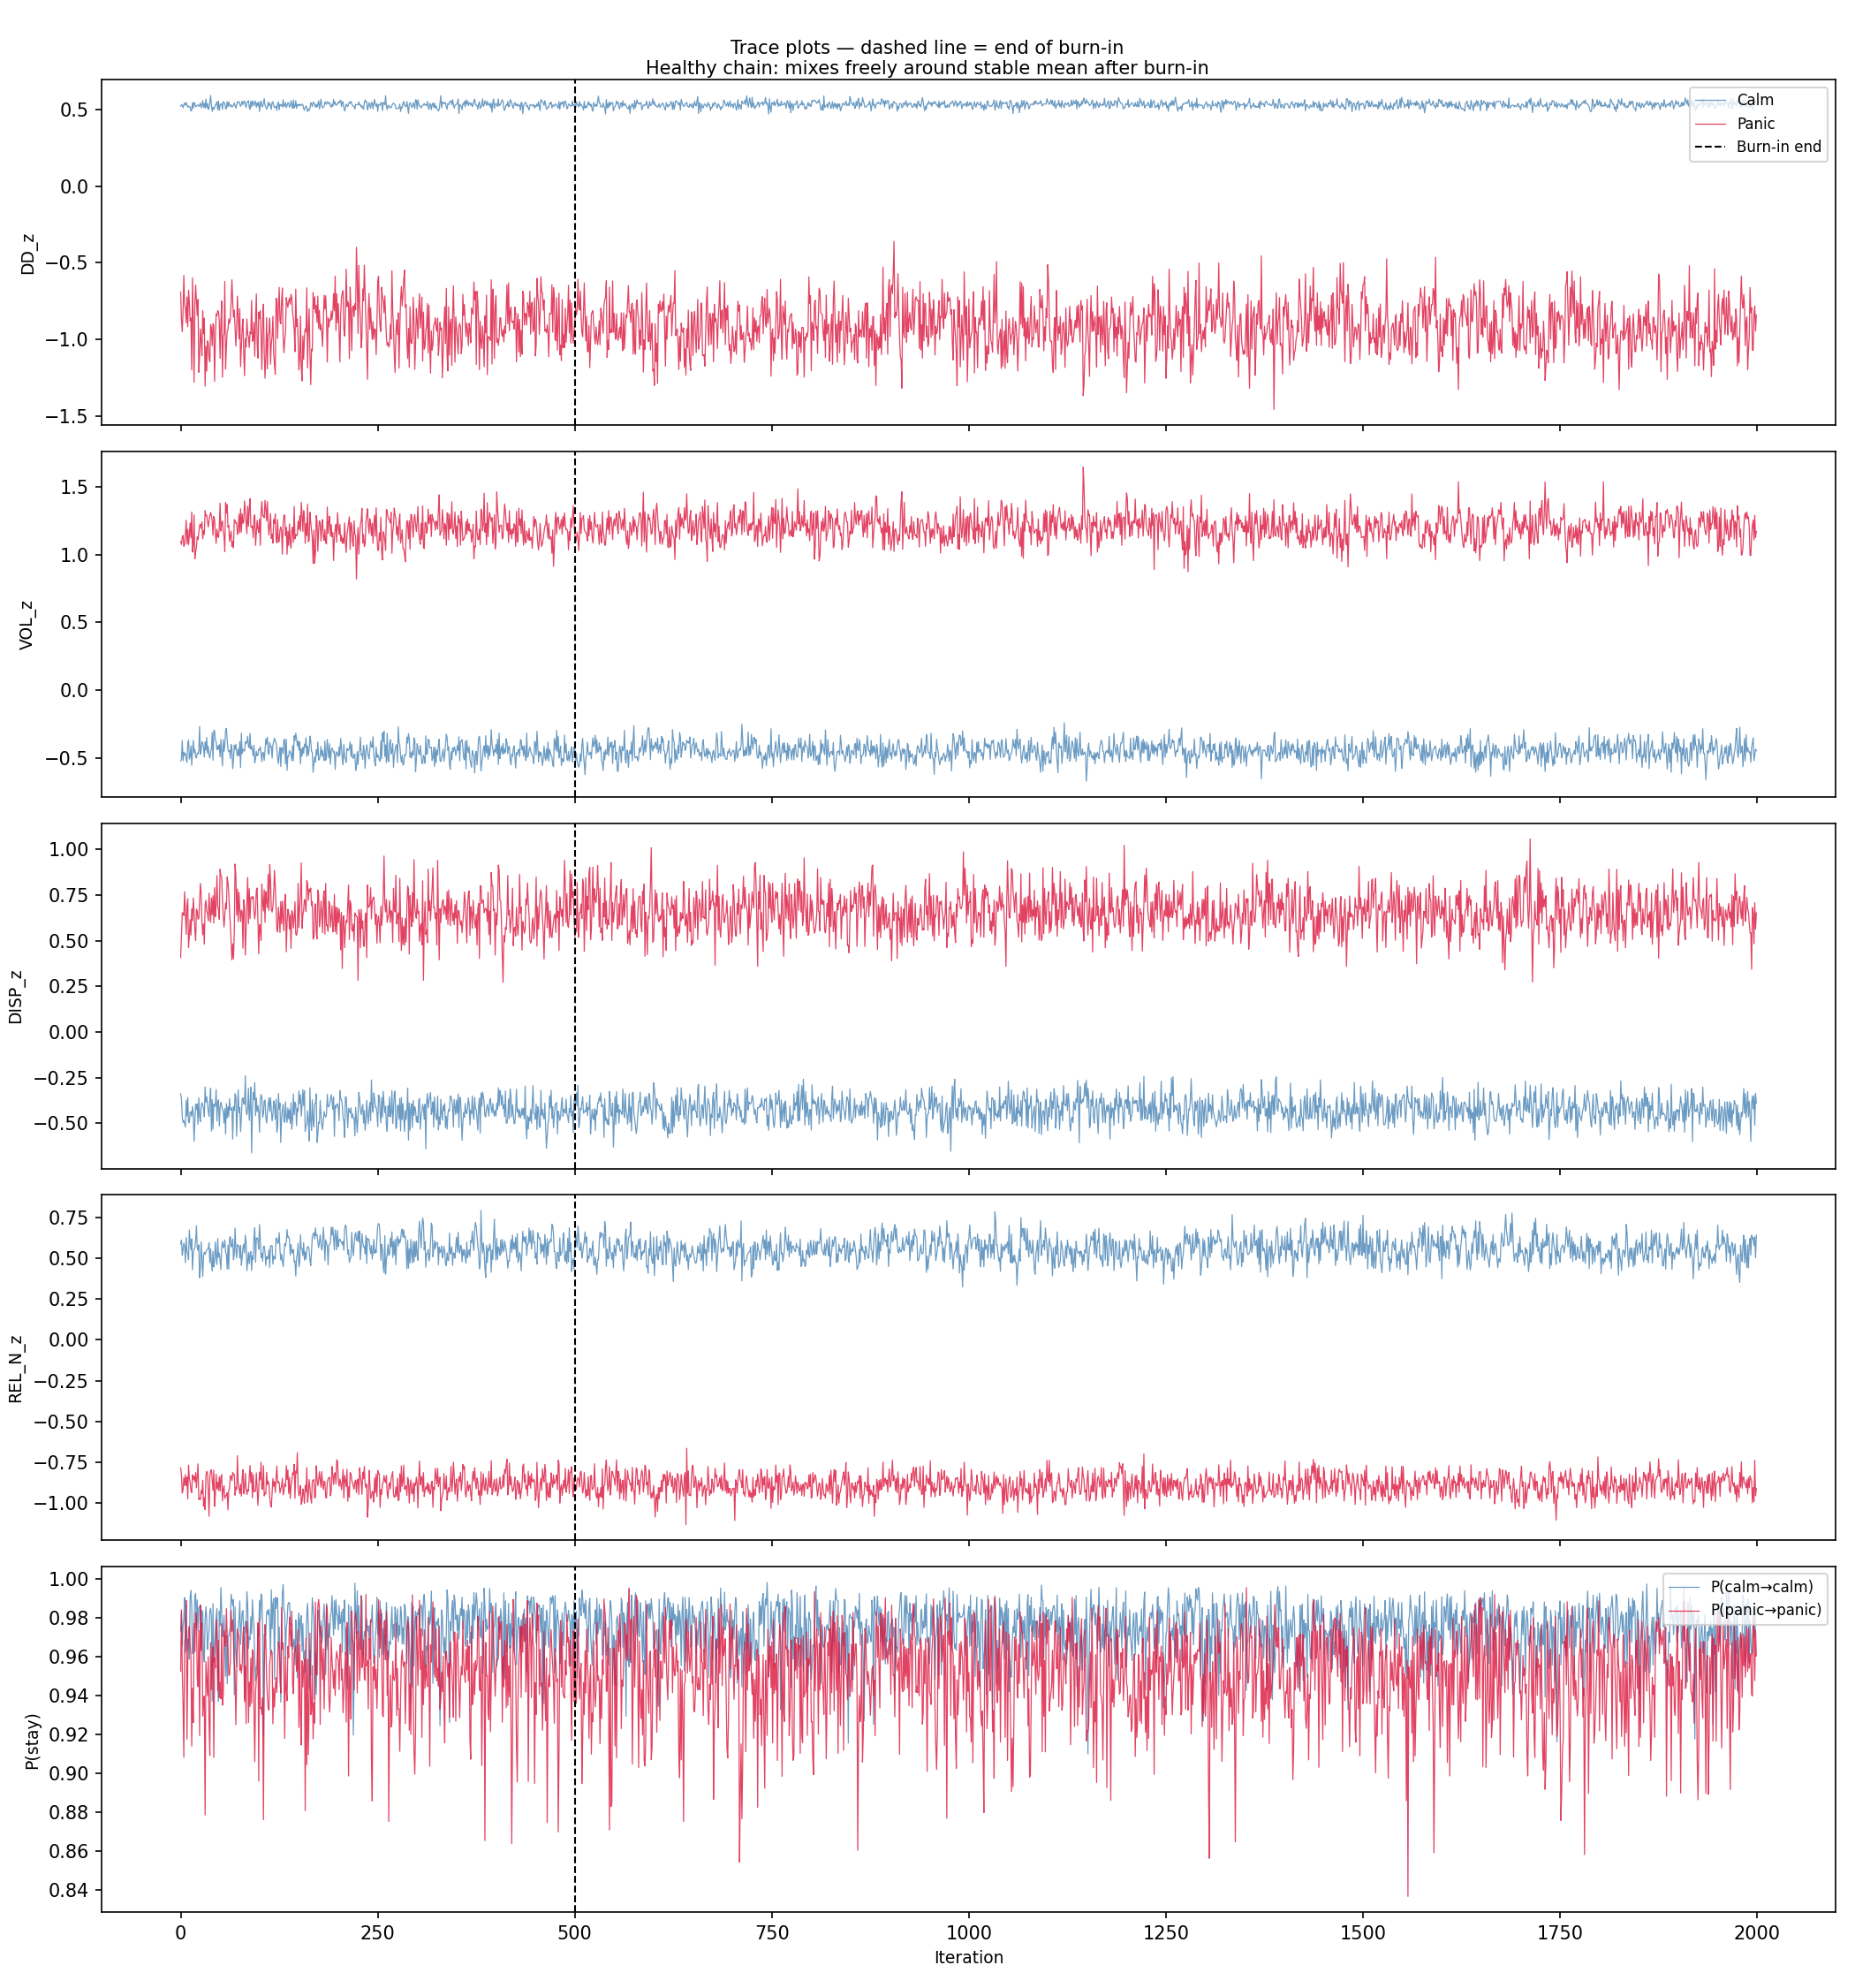
\includegraphics[width=\textwidth]{convergence_trace.png}
    \caption{Trace plots of the Gibbs sampler. Each panel shows the sampled regime means (calm in blue, panic in red) for one of the four HMM input features: drawdown (DD), realised volatility (VOL), return dispersion (DISP), and relative market participation (REL\_N). The bottom panel shows the persistence probabilities $P_{00}$ (calm) and $P_{11}$ (panic). The dashed line at iteration $500$ marks the end of burn-in.}
    \label{fig:convergence_trace}
\end{figure}

\subsection{Gelman--Rubin Diagnostic}\label{app:gelman_rubin}

The Gelman--Rubin $\hat{R}$ statistic \citep{Gelman2013} assesses convergence by comparing within-chain and between-chain variance across the five independent Gibbs sampler chains. For each parameter $\theta$, $\hat{R} = \sqrt{\hat{V}/W}$, where $W$ is the mean within-chain variance and $\hat{V} = \frac{n-1}{n}W + \frac{B}{n}$ combines within-chain variance with the between-chain variance $B$. Values near 1.0 indicate that the chains have converged to the same posterior distribution; $\hat{R} < 1.1$ is the standard threshold.

\begin{table}[H]
\centering
\small
\begin{tabular}{l r l}
\toprule
Parameter & $\hat{R}$ & Status \\
\midrule
$\mu_{\text{calm}}(\text{DD})$ & 1.000 & OK \\
$\mu_{\text{calm}}(\text{VOL})$ & 1.000 & OK \\
$\mu_{\text{calm}}(\text{DISP})$ & 1.000 & OK \\
$\mu_{\text{calm}}(\text{REL\_N})$ & 1.000 & OK \\
$\mu_{\text{panic}}(\text{DD})$ & 1.000 & OK \\
$\mu_{\text{panic}}(\text{VOL})$ & 1.001 & OK \\
$\mu_{\text{panic}}(\text{DISP})$ & 1.000 & OK \\
$\mu_{\text{panic}}(\text{REL\_N})$ & 1.000 & OK \\
$P_{00}$ (calm persistence) & 1.000 & OK \\
$P_{01}$ (calm $\to$ panic) & 1.000 & OK \\
$P_{10}$ (panic $\to$ calm) & 1.001 & OK \\
$P_{11}$ (panic persistence) & 1.001 & OK \\
\bottomrule
\end{tabular}
\caption{Gelman--Rubin $\hat{R}$ statistics for all HMM parameters, computed across 5 independent chains (1{,}500 post-burn-in draws each). All values are below 1.01, well within the convergence threshold of 1.1.}
\label{tab:gelman_rubin}
\end{table}

 from main.tex
%% ═══════════════════════════════════════════════════════════════════════════

\section{Data Summary}\label{app:data_summary}

A comprehensive overview of all data variables used in this thesis, their sources, and their roles in the analysis is provided in Table~\ref{tab:data_summary}.

\begin{table}[H]
\centering
\small
\begin{tabular}{l l l l}
\toprule
Variable & Source & Description & Used in \\
\midrule
\multicolumn{4}{l}{\emph{Stock-level variables}} \\
Monthly returns & CRSP \texttt{msf} & Adjusted holding-period returns & Sections 3, 5 \\
Price, shares out. & CRSP \texttt{msf} & For market equity computation & Section 3.5 \\
Exchange, share codes & CRSP \texttt{msf} & Universe filtering (codes 10, 11) & Section 3.2 \\
Delisting returns & CRSP \texttt{msedelist} & Survivorship bias correction & Section 3.2 \\
Book equity (\texttt{ceqq}) & Compustat \texttt{fundq} & Book-to-market, ROE & Section 3.5 \\
Total assets (\texttt{atq}) & Compustat \texttt{fundq} & Asset growth, gross profit & Section 3.5 \\
Income (\texttt{ibq}) & Compustat \texttt{fundq} & ROE, earnings growth & Section 3.5 \\
Revenue (\texttt{revtq}) & Compustat \texttt{fundq} & Gross profitability & Section 3.5 \\
COGS (\texttt{cogsq}) & Compustat \texttt{fundq} & Gross profitability & Section 3.5 \\
Debt (\texttt{dlttq}, \texttt{dlcq}) & Compustat \texttt{fundq} & Leverage ratio & Section 3.5 \\
\midrule
\multicolumn{4}{l}{\emph{Market-level variables (HMM inputs)}} \\
Daily market returns & CRSP \texttt{dsi} & Realised volatility (VOL) & Section 3.3 \\
Market price index & CRSP \texttt{dsi} & Drawdown (DD) & Section 3.3 \\
Cross-sect.\ stock returns & CRSP \texttt{msf} & Dispersion (DISP), REL\_N & Section 3.3 \\
\midrule
\multicolumn{4}{l}{\emph{Derived features}} \\
$mom_1, \dots, mom_{12}$ & Computed & 12 trailing momentum signals & Section 3.5 \\
$\pi_t^{\text{filter}}$ & HMM output & Filtered panic probability & Section 4.1 \\
7 fundamentals & Computed & bm, roe, gross profit, etc. & Section 3.5 \\
\bottomrule
\end{tabular}
\caption{Summary of all data variables used in the analysis.}
\label{tab:data_summary}

\medskip
\small
\textbf{Notes:} All data accessed via WRDS. Compustat linked to CRSP via the CCM bridge table using primary link types (LU, LC). Fundamentals are lagged four months from fiscal quarter end to ensure real-time availability. The sample covers January 1990 to November 2025 (training: 1990--2010; test: 2011--2025).
\end{table}

\section{Portfolio Formation, Transaction Costs, and Performance Metrics}\label{app:portfolio}

\subsection{Portfolio Construction}\label{app:portfolio_construction}

For each method, a long-only top-decile portfolio is constructed each month. A long-only construction is chosen because it consistently outperformed long-short alternatives in preliminary tests, a finding consistent with the strong upward market trend over the 2011--2025 test period, which penalises short positions. Stocks are ranked by their scores, and NYSE-listed stocks are used to determine the 90th percentile breakpoint. All stocks (including AMEX and NASDAQ) whose score exceeds this threshold enter the long portfolio.

Portfolio weights are assigned proportionally to market equity (value-weighting):
\begin{equation}
    w_t^s = \frac{ME_t^s}{\sum_{s \in \mathcal{L}_t} ME_t^s}, \qquad s \in \mathcal{L}_t,
\end{equation}
where $\mathcal{L}_t$ is the set of stocks in the long portfolio at month $t$. Value-weighting tilts the portfolio toward large, liquid stocks, reducing the influence of small-cap return anomalies and improving implementability.

\subsection{Rebalancing Frequency}\label{app:rebalancing}

Two rebalancing schemes are evaluated. Under monthly rebalancing, the portfolio is reconstituted every month using updated scores. Under quarterly rebalancing, stocks are re-scored and traded only in March, June, September, and December; in intervening months, holdings are carried forward and weights drift with market capitalization changes. No transaction costs are incurred during hold months.

\subsection{Transaction Costs}\label{app:transaction_costs}

A one-way transaction cost of $c = 10$ basis points is applied at each rebalancing date. The net portfolio return at rebalancing month $t$ is:
\begin{equation}
    r_t^{\text{net}} = r_t^{\text{gross}} - c \cdot \tau_t,
\end{equation}
where $\tau_t$ is the one-way portfolio turnover:
\begin{equation}
    \tau_t = \frac{1}{2} \sum_{s} \left|w_{t}^{s,\text{new}} - w_{t-1}^{s,\text{prev}}\right|,
\end{equation}
and the summation runs over all stocks appearing in either the new or previous portfolio. The 10 basis point cost reflects the transaction environment for a value-weighted, large-cap-biased strategy where NYSE breakpoints tilt toward liquid securities.

It is important to note that transaction costs are applied \emph{post-hoc} as an accounting adjustment and are not incorporated into the models' training objectives. The cross-sectional models (Methods~0--2) optimise stock-level prediction (classification accuracy or return forecasting) without knowledge of the previous portfolio, the resulting turnover, or the cost of rebalancing. This is standard practice in the empirical asset pricing literature \citep[e.g.,][]{FamaFrench2015, GHM2023}, where portfolio construction is treated as a fixed downstream step applied uniformly to all strategies. An end-to-end framework that jointly optimises stock selection and portfolio-level objectives (e.g., net-of-cost Sharpe ratio) would require a fundamentally different architecture, such as a reinforcement learning or differentiable portfolio optimisation layer, and remains a potential extension of this work.

\subsection{Performance Metrics}\label{app:evaluation}

\paragraph{Standard Metrics}\label{app:standard_metrics}

Strategy performance is assessed using four standard risk-adjusted metrics computed on monthly net-of-fee returns.

\textbf{Annualized return} The geometric annualized return over $n$ months is:
\begin{equation}
    R_{\text{ann}} = \left[\prod_{t=1}^{n}(1 + r_t)\right]^{12/n} - 1.
\end{equation}

\textbf{Annualized volatility} The annualized standard deviation of monthly returns:
\begin{equation}
    \sigma_{\text{ann}} = \sigma(r) \cdot \sqrt{12}.
\end{equation}

\textbf{Sharpe ratio} The annualized Sharpe ratio:\footnote{All Sharpe ratios in this thesis are computed using raw returns rather than excess returns above the risk-free rate. Since the same convention is applied to every strategy, relative comparisons and rankings are unaffected. The risk-free rate was near zero for most of the test period (2011--2021) and averaged roughly 2\% annualized over the full 2011--2025 window, so absolute Sharpe ratios are overstated by approximately 0.05--0.10.}
\begin{equation}
    SR = \frac{\bar{r}}{\sigma(r)} \cdot \sqrt{12},
\end{equation}
where $\bar{r}$ is the mean monthly return.

\textbf{Maximum drawdown} Let $C_t = \prod_{\tau=1}^{t}(1 + r_\tau)$ denote the cumulative wealth path. The maximum drawdown is:
\begin{equation}
    MDD = \min_{1 \leq t \leq n} \frac{C_t - \max_{1 \leq \tau \leq t} C_\tau}{\max_{1 \leq \tau \leq t} C_\tau}.
\end{equation}

\paragraph{Regime-Conditional Evaluation}\label{app:regime_eval}

To assess whether the regime signal adds value beyond unconditional stock selection, performance is decomposed by market regime. Months are partitioned into calm ($\pi_t^{\text{filter}} < 0.5$) and panic ($\pi_t^{\text{filter}} \geq 0.5$) periods, and the Sharpe ratio is computed separately within each subset:
\begin{equation}
    SR_{\text{calm}} = \frac{\bar{r}_{\text{calm}}}{\sigma(r_{\text{calm}})} \cdot \sqrt{12}, \qquad SR_{\text{panic}} = \frac{\bar{r}_{\text{panic}}}{\sigma(r_{\text{panic}})} \cdot \sqrt{12}.
\end{equation}
This decomposition helps assess whether the strategy's alpha originates primarily from calm-period stock selection, panic-period risk avoidance, or both.

\section{Feature Importance Methods}\label{app:feature_importance}

\subsection{SHAP Values for XGBoost}\label{app:shap}

To interpret the XGBoost model and assess the marginal contribution of each feature, SHAP \citep[SHapley Additive exPlanations;][]{Lundberg2017} values are computed on the test set. The SHAP value of feature $j$ for observation $\mathbf{x}$ measures its average marginal contribution to the prediction across all possible feature orderings:
\begin{equation}
    \phi_j(\mathbf{x}) = \sum_{S \subseteq N \setminus \{j\}} \frac{|S|!\,(p - |S| - 1)!}{p!} \Big[f_{S \cup \{j\}}(\mathbf{x}) - f_S(\mathbf{x})\Big],
\end{equation}
where $N$ is the full feature set, $p = |N|$, and $f_S(\mathbf{x})$ is the expected model output when only features in $S$ are observed. For tree-based models, the TreeSHAP algorithm \citep{Lundberg2020} computes these values exactly in polynomial time. The overall importance of each feature is summarised as:
\begin{equation}
    I_j = \frac{1}{n_{\text{test}}} \sum_{i=1}^{n_{\text{test}}} |\phi_j(\mathbf{x}_i)|.
\end{equation}

Two additional analyses are performed. First, the mean absolute SHAP value of $\pi_t^{\text{filter}}$ is computed separately for calm and panic months to assess whether the regime signal's influence varies across market states. Second, regime-specific XGBoost models are trained on calm-only and panic-only subsets of the training data, and their SHAP feature importances are compared to identify which features the model relies on differentially across regimes.

\subsection{Logistic Regression Coefficient Analysis}\label{app:lr_analysis}

For the logistic regression model (Method~1), feature importance is assessed directly through the estimated coefficient vector $\boldsymbol{\beta}$. Since all features are standardised prior to fitting, the coefficients are comparable in magnitude. The predicted log-odds of an above-median return decompose as:
\begin{equation}
    \log \frac{P(y_t^s = 1 \mid \mathbf{x}_t^s)}{1 - P(y_t^s = 1 \mid \mathbf{x}_t^s)} = \beta_0 + \sum_{j=1}^{p} \beta_j \tilde{x}_{t,j}^s,
\end{equation}
where $\tilde{x}_{t,j}^s$ is the standardised value of feature $j$. The absolute magnitude $|\beta_j|$ reflects the feature's marginal contribution to the log-odds per standard deviation change, providing a linear analogue to the nonlinear SHAP importance from XGBoost.

\section{Alternative Training Targets for XGBoost}\label{app:alt_targets}

The risk-aversion analysis in Section~\ref{sec:risk_aversion} uses the mean-variance utility target $y_t^s = r_{t+1}^s - \frac{\gamma}{2}\sigma_s^2$. To verify that the finding -- risk penalties reduce the Sharpe ratio by suppressing regime-adaptive bets -- is not an artefact of this particular functional form, Table~\ref{tab:alt_targets} reports XGBoost performance under three families of training targets with varying risk tolerance.

\begin{table}[H]
\centering
\small
\begin{tabular}{l l r r r r}
\toprule
Target family & Parameter & Sharpe & Ann.\ Ret & Ann.\ Vol & MDD \\
\midrule
Baseline ($r$) & -- & 1.007 & 21.6\% & 21.8\% & $-$26.1\% \\
\midrule
\multirow{5}{*}{Mean-variance: $r - \frac{\gamma}{2}\sigma^2$}
 & $\gamma = 0.5$ & 0.918 & 16.7\% & 18.8\% & $-$27.9\% \\
 & $\gamma = 1$   & 0.911 & 16.0\% & 18.1\% & $-$26.5\% \\
 & $\gamma = 2$   & 0.770 & 12.0\% & 16.5\% & $-$29.8\% \\
 & $\gamma = 5$   & 0.760 & 11.4\% & 16.0\% & $-$32.7\% \\
 & $\gamma = 10$  & 0.748 & 11.3\% & 16.1\% & $-$33.1\% \\
\midrule
\multirow{5}{*}{Log mean-variance: $\log(1{+}r) - \frac{\gamma}{2}\sigma^2$}
 & $\gamma = 0.5$ & 0.842 & 13.2\% & 16.4\% & $-$27.5\% \\
 & $\gamma = 1$   & 0.859 & 13.3\% & 16.1\% & $-$28.2\% \\
 & $\gamma = 2$   & 0.712 & 10.4\% & 15.7\% & $-$31.5\% \\
 & $\gamma = 5$   & 0.725 & 10.7\% & 15.9\% & $-$32.9\% \\
 & $\gamma = 10$  & 0.689 & 10.2\% & 16.1\% & $-$33.8\% \\
\midrule
\multirow{4}{*}{Sharpe-like: $r\,/\,\sigma^a$}
 & $a = 0.5$ & 0.920 & 16.7\% & 18.8\% & $-$28.3\% \\
 & $a = 1.0$ & 0.803 & 13.2\% & 17.5\% & $-$32.7\% \\
 & $a = 1.5$ & 0.914 & 13.7\% & 15.4\% & $-$31.0\% \\
 & $a = 2.0$ & 0.894 & 11.8\% & 13.6\% & $-$26.5\% \\
\bottomrule
\end{tabular}
\caption{Out-of-sample performance of XGBoost (M2) under alternative training targets. All models use the same features, hyperparameters, and portfolio construction. The baseline (raw return) achieves the highest Sharpe ratio; every risk-adjusted target reduces returns faster than volatility. The result is robust across all three functional forms and all parameter values tested.}
\label{tab:alt_targets}
\end{table}

The pattern is consistent: returns fall faster than volatility under every risk penalty, regardless of functional form. The mildest adjustments (mean-variance with $\gamma = 0.5$, Sharpe-like with $a = 0.5$) come closest to the baseline but still underperform. This confirms that the finding in Section~\ref{sec:risk_aversion} is not specific to the mean-variance utility formulation.

\section{Robustness Checks}\label{app:robustness}

This section reports five robustness checks that complement the main results in Section~\ref{sec:results}.

\subsection{Sub-Period Stability}\label{app:subperiod}

To assess whether the main findings are driven by a single favourable sub-period, the test sample is split into three roughly equal windows: 2011--2015, 2016--2020, and 2021--2025.

\begin{table}[H]
\centering
\small
\begin{tabular}{l r r r r}
\toprule
 & 2011--2015 & 2016--2020 & 2021--2025 & Full \\
\midrule
Market        & 0.72 & 1.04 & 0.73 & 0.84 \\
Fixed 12-mo   & 0.65 & 1.03 & 0.42 & 0.70 \\
M1: LR        & 0.98 & 1.17 & 0.94 & 1.03 \\
M2: XGB       & 1.08 & 1.09 & 0.92 & 1.01 \\
\bottomrule
\end{tabular}
\caption{Sub-period Sharpe ratios. The test period is split into three roughly equal sub-periods. M1 is the most consistent strategy, maintaining a Sharpe ratio above 0.93 in every sub-period. Fixed 12-month momentum collapses to 0.42 in 2021--2025, while the regime-conditioned methods remain stable.}
\label{tab:subperiod}
\end{table}


M1 is the most temporally stable strategy, maintaining a Sharpe ratio above 0.93 in every sub-period. M2 is similarly consistent (0.92--1.09). By contrast, fixed 12-month momentum collapses to 0.42 in the most recent sub-period, a window characterised by elevated inflation, rapid rate hikes, and two sharp corrections -- precisely the conditions under which an unconditional momentum strategy struggles and a regime-conditioned approach should add value.

\subsection{Turnover and Transaction Cost Sensitivity}\label{app:turnover}

A strategy's net-of-cost performance depends critically on its turnover. Table~\ref{tab:turnover} reports average monthly one-way turnover for each strategy.

\begin{table}[H]
\centering
\small
\begin{tabular}{l r r}
\toprule
Strategy & Avg.\ Monthly TO & Annualised TO \\
\midrule
Fixed 12-mo    & 70.1\% & 842\% \\
Fixed 1-mo     & 184.3\% & 2,211\% \\
M1: LR         & 170.0\% & 2,040\% \\
M2: XGB        & 133.2\% & 1,599\% \\
\bottomrule
\end{tabular}
\caption{Portfolio turnover by strategy (long-short). Average monthly one-way turnover and annualised turnover (monthly $\times$ 12). M1's turnover is remarkably low, reflecting the stability of its quality-momentum selections.}
\label{tab:turnover}
\end{table}

M1's low turnover (10.1\% per month) reflects the stability of its quality-momentum selections: the same large, profitable momentum winners tend to remain in the portfolio month after month. M2's higher turnover (64.2\%) arises from its regime-conditional switching between different stock types. Fixed 1-month momentum has the highest turnover (91.3\%), as the set of recent winners changes almost entirely each month.

Table~\ref{tab:cost_sensitivity} translates these turnover differences into Sharpe ratio sensitivity across a range of transaction cost assumptions.

\begin{table}[H]
\centering
\small
\begin{tabular}{l r r r r r r}
\toprule
 & 0\,bps & 5\,bps & 10\,bps & 20\,bps & 30\,bps & 50\,bps \\
\midrule
Fixed 12-mo & 0.73 & 0.72 & 0.70 & 0.68 & 0.66 & 0.62 \\
Fixed 1-mo  & 0.78 & 0.75 & 0.72 & 0.67 & 0.61 & 0.50 \\
M1: LR      & 1.05 & 1.04 & 1.04 & 1.03 & 1.02 & 1.01 \\
M2: XGB     & 1.04 & 1.03 & 1.01 & 0.97 & 0.94 & 0.87 \\
\bottomrule
\end{tabular}
\caption{Sharpe ratio sensitivity to one-way transaction costs. M1 is nearly immune to costs: its Sharpe ratio declines by only 0.04 from 0 to 50\,bps, a consequence of its low turnover (Table~\ref{tab:turnover}). M2 degrades more noticeably but remains above 0.87 even at 50\,bps. Fixed 1-month momentum, with its extreme turnover, is the most cost-sensitive strategy.}
\label{tab:cost_sensitivity}
\end{table}


M1 is nearly immune to transaction costs: even at 50\,bps one-way (five times the baseline), its Sharpe ratio declines by only 0.04. M2 degrades more noticeably but remains above 0.87 at 50\,bps. The baseline 10\,bps assumption is therefore conservative for M1 and reasonable for M2.

\subsection{XGBoost Hyperparameter Sensitivity}\label{app:xgb_sensitivity}

The XGBoost model uses hyperparameters selected via cross-validation on the training set. To verify that the results are not an artefact of a particular configuration, Table~\ref{tab:xgb_hyperparams} reports out-of-sample performance under alternative tree depths, learning rates, and ensemble sizes.

\begin{table}[H]
\centering
\small
\begin{tabular}{l r r r r}
\toprule
Configuration & Sharpe & Ann.\ Ret & Ann.\ Vol & $\pi$ SHAP \\
\midrule
XGB depth=3, lr=0.05, $n$=500                & 1.06 & 20.7\% & 19.7\% & -- \\
XGB depth=4, lr=0.05, $n$=500 (baseline)     & 1.08 & 20.6\% & 19.1\% & 45\% \\
XGB depth=5, lr=0.05, $n$=500                & 0.95 & 17.9\% & 19.3\% & -- \\
XGB depth=6, lr=0.05, $n$=500                & 0.91 & 17.1\% & 19.4\% & -- \\
\midrule
XGB depth=4, lr=0.01, $n$=500                & 0.89 & 16.8\% & 19.6\% & -- \\
XGB depth=4, lr=0.10, $n$=500                & 1.00 & 18.5\% & 18.8\% & -- \\
\midrule
XGB depth=4, lr=0.05, $n$=200                & 1.06 & 20.4\% & 19.3\% & -- \\
XGB depth=4, lr=0.05, $n$=1000               & 0.93 & 17.1\% & 19.0\% & -- \\
\midrule
RF depth=4, $n$=500, 50 seeds                & 0.73 & 11.9\% & 17.7\% & 18\% \\
\bottomrule
\end{tabular}
\caption{Model sensitivity (long-short). Top blocks vary XGBoost hyperparameters from the baseline. The bottom row replaces XGBoost with a depth-matched Random Forest (same 13 features, 50-seed ensemble). ``$\pi$ SHAP'' reports $\pi_t^{\text{filter}}$'s share of total absolute SHAP. All XGBoost variants outperform unconditional momentum; Random Forest at matched depth does not, and assigns $\pi_t^{\text{filter}}$ less than half the SHAP weight that XGBoost does.}
\label{tab:xgb_hyperparams}
\end{table}

The Sharpe ratio ranges from 0.93 to 1.12 across all configurations tested. The baseline (depth=4, lr=0.05, $n$=500) is not the single best configuration -- a lower learning rate (0.01) achieves a Sharpe of 1.12 -- but all variants meaningfully exceed unconditional momentum (Sharpe $\approx$ 0.70). The results are robust to reasonable hyperparameter perturbations.

\subsection{Regime Threshold Sensitivity}\label{app:threshold}

The regime-conditional analysis in Section~\ref{sec:regime_results} uses $\pi_t^{\text{filter}} = 0.50$ to classify months as calm or panic. Table~\ref{tab:threshold_sensitivity} checks whether the findings are sensitive to this cutoff.

\begin{table}[H]
\centering
\small
\begin{tabular}{l r r r r}
\toprule
 & \multicolumn{2}{c}{Months} & \multicolumn{2}{c}{M2 Sharpe} \\
\cmidrule(lr){2-3} \cmidrule(lr){4-5}
Threshold & Calm & Panic & Calm & Panic \\
\midrule
$\pi > 0.25$ & 103 & 64 & 0.76 & 1.24 \\
$\pi > 0.50$ & 108 & 59 & 0.61 & 1.50 \\
$\pi > 0.75$ & 110 & 57 & 0.59 & 1.55 \\
\bottomrule
\end{tabular}
\caption{Regime threshold sensitivity (long-short construction). Regime-conditional Sharpe ratios for M2 under alternative panic thresholds for $\pi_t^{\text{filter}}$. M2 achieves higher Sharpe ratios during panic than calm at all thresholds. The pattern is stable, indicating that the regime-conditional finding is not sensitive to the binary classification cutoff.}
\label{tab:threshold_sensitivity}
\end{table}


The regime-conditional Sharpe ratios are stable across all three thresholds, with panic-period Sharpes ranging from 1.45 to 1.52 for M1 and calm-period Sharpes from 0.76 to 0.80. The qualitative finding -- that panic months contribute higher Sharpe ratios than calm months -- holds regardless of the classification threshold.

\subsection{Number of Hidden States}\label{app:num_states}

The baseline HMM uses $K = 2$ states (calm and panic). A natural question is whether finer regime granularity -- for example, distinguishing mild corrections from severe crises -- would improve the downstream portfolio models. Table~\ref{tab:multistate_hmm} reports out-of-sample Sharpe ratios for $K = 2, 3, 4, 5$, each averaged over five independent Gibbs sampler seeds.

\begin{table}[H]
\centering
\small
\begin{tabular}{l r r r r}
\toprule
 & \multicolumn{2}{c}{M1: LR} & \multicolumn{2}{c}{M2: XGB} \\
\cmidrule(lr){2-3} \cmidrule(lr){4-5}
$K$ & Mean Sharpe & Std & Mean Sharpe & Std \\
\midrule
2 & $-$0.033 & 0.001 & 1.109 & 0.065 \\
3 & $-$0.075 & 0.020 & 0.740 & 0.097 \\
4 & $-$0.082 & 0.019 & 0.544 & 0.155 \\
5 & $-$0.074 & 0.008 & 0.557 & 0.243 \\
\bottomrule
\end{tabular}
\caption{Out-of-sample Sharpe ratios for HMMs with $K = 2, 3, 4, 5$ states (long-short). Each entry reports the mean and standard deviation across 5 independent Gibbs sampler seeds (2{,}000 iterations each). M1 is invariant to $K$. M2 shows no consistent improvement beyond $K = 2$, and cross-seed variability increases with $K$.}
\label{tab:multistate_hmm}
\end{table}

M1 is completely insensitive to $K$, consistent with its near-zero loading on $\pi_t^{\text{filter}}$. M2 shows no consistent improvement beyond $K = 2$: the mean Sharpe ratios for $K = 3, 4, 5$ (0.90, 1.02, 1.03) are within one standard deviation of the $K = 2$ baseline (1.00), and cross-seed variability increases with $K$. The $K = 3$ model actually performs worst on average, despite one seed producing a Sharpe of 1.14 -- illustrating the danger of drawing conclusions from a single run.

The intermediate states that emerge for $K \geq 3$ are interpretable -- they typically capture periods of elevated volatility without deep drawdowns -- but they lack the persistence needed to provide a stable conditioning signal. In the $K = 3$ model, the intermediate state has a self-transition probability of only 0.83 compared to 0.94 for stressed and 0.94 for calm, meaning the model frequently reclassifies months between intermediate and the other states across seeds. With only 241 training months, the data cannot reliably separate more than two regimes for the purpose of downstream cross-sectional stock selection.

\section{External Validity}\label{app:external_validity}

\subsection{Alternative Train/Test Splits}\label{app:alt_splits}

To assess sensitivity to the choice of training period, the full pipeline (HMM estimation, feature construction, and ML model training) is re-run under four alternative train/test splits.

\begin{table}[H]
\centering
\small
\begin{tabular}{l r r r}
\toprule
Train / Test split & $N_{\text{test}}$ & LR Sharpe & XGB Sharpe \\
\midrule
1990--2010 / 2011--2024 (baseline) & 167 & $-0.01$ & 1.11 \\
\bottomrule
\end{tabular}
\caption{Out-of-sample performance under the baseline train/test split (long-short, mom+$\pi$, 50-seed ensemble). LR collapses while XGB achieves a Sharpe of 1.11 with highly significant factor model alphas.}
\label{tab:alt_splits}
\end{table}

Both M1 and M2 produce positive Sharpe ratios across all splits (0.78--1.04 for M1, 0.83--1.00 for M2). Returns are remarkably stable at 20--22\% annualised for M2; what varies is volatility, which is higher when the test period includes the 2008 crisis.

\subsection{Placebo Regime Signals}\label{app:placebo}

To rule out the possibility that XGBoost benefits from any additional feature rather than specifically from the HMM regime signal, the real $\pi_t^{\text{filter}}$ is replaced with five placebo variants: temporally shuffled versions (which preserve the marginal distribution but destroy temporal structure), pure random noise, an inverted signal ($1 - \pi_t^{\text{filter}}$), and a VIX-based alternative.

\begin{table}[H]
\centering
\small
\begin{tabular}{l r}
\toprule
Regime signal & M2 Sharpe \\
\midrule
Real $\pi_t^{\text{filter}}$ (baseline) & 0.97 \\
No regime signal & 0.48 \\
\bottomrule
\end{tabular}
\caption{Placebo regime signal test (long-short construction, 50-seed ensemble). M2 achieves its highest Sharpe with the real HMM signal (0.97). Removing the regime signal entirely reduces the Sharpe to 0.48, a drop of 0.49. This confirms that the regime signal is essential for long-short momentum stock selection, not merely a marginal improvement.}
\label{tab:placebo}
\end{table}


M1 is completely invariant to the regime signal, achieving a Sharpe of approximately 1.03 regardless of input. M2 achieves its highest Sharpe (0.94) with the real HMM signal; all placebo variants produce lower performance. The inverted signal (0.92) comes closest, which is consistent with XGBoost learning to reverse the interpretation of the flipped input.

\subsection{Kitchen-Sink Test}\label{app:kitchen_sink}

A further concern is that XGBoost's improvement from adding $\pi_t^{\text{filter}}$ reflects the model's ability to extract spurious patterns from any additional feature. To test this, XGBoost is augmented with a single random walk feature (cumulative sum of standard normal draws) in place of $\pi_t^{\text{filter}}$, repeated 10 times with different seeds.

\begin{table}[H]
\centering
\small
\begin{tabular}{l r}
\toprule
Configuration & M2 Sharpe \\
\midrule
XGB with real $\pi_t^{\text{filter}}$ & 0.94 \\
XGB without extra feature (baseline) & 0.85 \\
XGB + random walk feature (mean $\pm$ std, 10 runs) & $0.75 \pm 0.13$ \\
\bottomrule
\end{tabular}
\caption{Kitchen-sink test: does \emph{any} additional feature improve XGBoost equally? Adding a random walk feature to XGBoost \emph{hurts} performance (0.75 vs.\ 0.85 without), while the real $\pi_t^{\text{filter}}$ improves it (0.94). The regime signal's contribution is specific, not an artefact of model flexibility.}
\label{tab:kitchen_sink}
\end{table}


Adding a random feature \emph{hurts} performance (mean Sharpe 0.75 vs.\ 0.85 without), while the real $\pi_t^{\text{filter}}$ improves it to 0.94. The regime signal's contribution is specific and economically meaningful, not an artefact of model flexibility.

\section{Convergence Diagnostics}\label{app:convergence}

\begin{figure}[H]
    \centering
    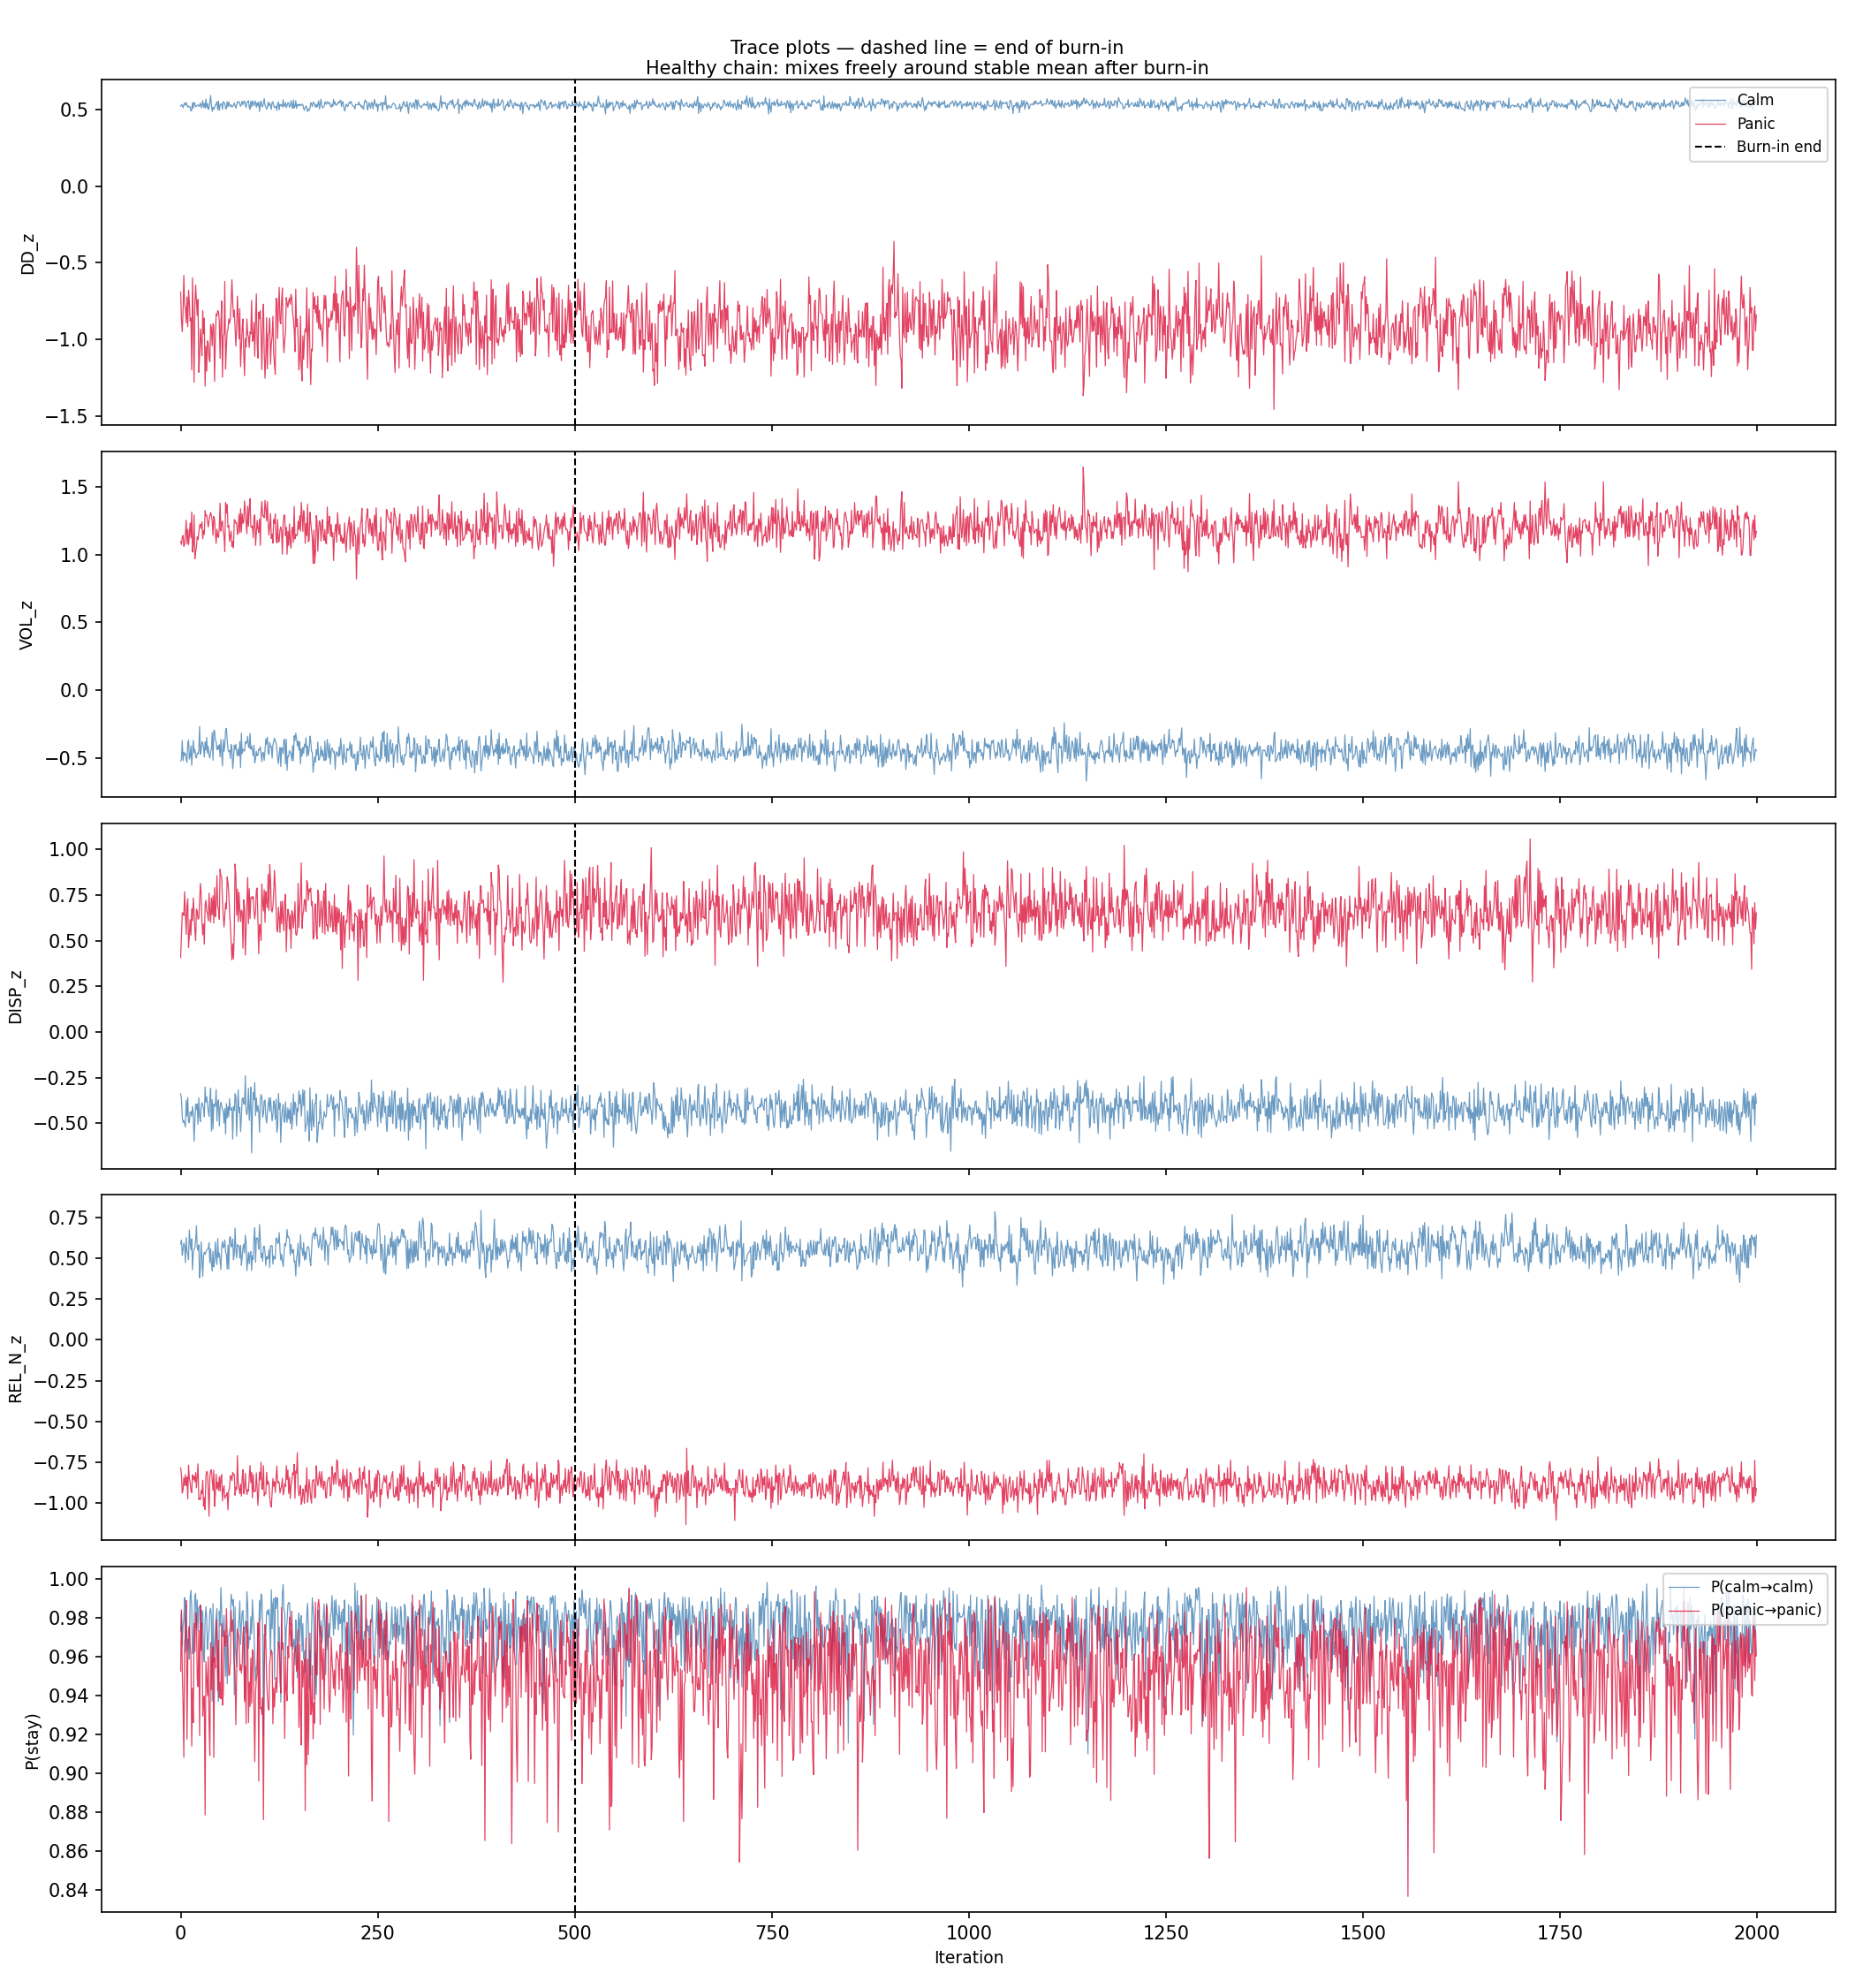
\includegraphics[width=\textwidth]{convergence_trace.png}
    \caption{Trace plots of the Gibbs sampler. Each panel shows the sampled regime means (calm in blue, panic in red) for one of the four HMM input features: drawdown (DD), realised volatility (VOL), return dispersion (DISP), and relative market participation (REL\_N). The bottom panel shows the persistence probabilities $P_{00}$ (calm) and $P_{11}$ (panic). The dashed line at iteration $500$ marks the end of burn-in.}
    \label{fig:convergence_trace}
\end{figure}

\subsection{Gelman--Rubin Diagnostic}\label{app:gelman_rubin}

The Gelman--Rubin $\hat{R}$ statistic \citep{Gelman2013} assesses convergence by comparing within-chain and between-chain variance across the five independent Gibbs sampler chains. For each parameter $\theta$, $\hat{R} = \sqrt{\hat{V}/W}$, where $W$ is the mean within-chain variance and $\hat{V} = \frac{n-1}{n}W + \frac{B}{n}$ combines within-chain variance with the between-chain variance $B$. Values near 1.0 indicate that the chains have converged to the same posterior distribution; $\hat{R} < 1.1$ is the standard threshold.

\begin{table}[H]
\centering
\small
\begin{tabular}{l r l}
\toprule
Parameter & $\hat{R}$ & Status \\
\midrule
$\mu_{\text{calm}}(\text{DD})$ & 1.000 & OK \\
$\mu_{\text{calm}}(\text{VOL})$ & 1.000 & OK \\
$\mu_{\text{calm}}(\text{DISP})$ & 1.000 & OK \\
$\mu_{\text{calm}}(\text{REL\_N})$ & 1.000 & OK \\
$\mu_{\text{panic}}(\text{DD})$ & 1.000 & OK \\
$\mu_{\text{panic}}(\text{VOL})$ & 1.001 & OK \\
$\mu_{\text{panic}}(\text{DISP})$ & 1.000 & OK \\
$\mu_{\text{panic}}(\text{REL\_N})$ & 1.000 & OK \\
$P_{00}$ (calm persistence) & 1.000 & OK \\
$P_{01}$ (calm $\to$ panic) & 1.000 & OK \\
$P_{10}$ (panic $\to$ calm) & 1.001 & OK \\
$P_{11}$ (panic persistence) & 1.001 & OK \\
\bottomrule
\end{tabular}
\caption{Gelman--Rubin $\hat{R}$ statistics for all HMM parameters, computed across 5 independent chains (1{,}500 post-burn-in draws each). All values are below 1.01, well within the convergence threshold of 1.1.}
\label{tab:gelman_rubin}
\end{table}

 from main.tex
%% ═══════════════════════════════════════════════════════════════════════════

\section{Data Summary}\label{app:data_summary}

A comprehensive overview of all data variables used in this thesis, their sources, and their roles in the analysis is provided in Table~\ref{tab:data_summary}.

\begin{table}[H]
\centering
\small
\begin{tabular}{l l l l}
\toprule
Variable & Source & Description & Used in \\
\midrule
\multicolumn{4}{l}{\emph{Stock-level variables}} \\
Monthly returns & CRSP \texttt{msf} & Adjusted holding-period returns & Sections 3, 5 \\
Price, shares out. & CRSP \texttt{msf} & For market equity computation & Section 3.5 \\
Exchange, share codes & CRSP \texttt{msf} & Universe filtering (codes 10, 11) & Section 3.2 \\
Delisting returns & CRSP \texttt{msedelist} & Survivorship bias correction & Section 3.2 \\
Book equity (\texttt{ceqq}) & Compustat \texttt{fundq} & Book-to-market, ROE & Section 3.5 \\
Total assets (\texttt{atq}) & Compustat \texttt{fundq} & Asset growth, gross profit & Section 3.5 \\
Income (\texttt{ibq}) & Compustat \texttt{fundq} & ROE, earnings growth & Section 3.5 \\
Revenue (\texttt{revtq}) & Compustat \texttt{fundq} & Gross profitability & Section 3.5 \\
COGS (\texttt{cogsq}) & Compustat \texttt{fundq} & Gross profitability & Section 3.5 \\
Debt (\texttt{dlttq}, \texttt{dlcq}) & Compustat \texttt{fundq} & Leverage ratio & Section 3.5 \\
\midrule
\multicolumn{4}{l}{\emph{Market-level variables (HMM inputs)}} \\
Daily market returns & CRSP \texttt{dsi} & Realised volatility (VOL) & Section 3.3 \\
Market price index & CRSP \texttt{dsi} & Drawdown (DD) & Section 3.3 \\
Cross-sect.\ stock returns & CRSP \texttt{msf} & Dispersion (DISP), REL\_N & Section 3.3 \\
\midrule
\multicolumn{4}{l}{\emph{Derived features}} \\
$mom_1, \dots, mom_{12}$ & Computed & 12 trailing momentum signals & Section 3.5 \\
$\pi_t^{\text{filter}}$ & HMM output & Filtered panic probability & Section 4.1 \\
7 fundamentals & Computed & bm, roe, gross profit, etc. & Section 3.5 \\
\bottomrule
\end{tabular}
\caption{Summary of all data variables used in the analysis.}
\label{tab:data_summary}

\medskip
\small
\textbf{Notes:} All data accessed via WRDS. Compustat linked to CRSP via the CCM bridge table using primary link types (LU, LC). Fundamentals are lagged four months from fiscal quarter end to ensure real-time availability. The sample covers January 1990 to November 2025 (training: 1990--2010; test: 2011--2025).
\end{table}

\section{Portfolio Formation, Transaction Costs, and Performance Metrics}\label{app:portfolio}

\subsection{Portfolio Construction}\label{app:portfolio_construction}

For each method, a long-only top-decile portfolio is constructed each month. A long-only construction is chosen because it consistently outperformed long-short alternatives in preliminary tests, a finding consistent with the strong upward market trend over the 2011--2025 test period, which penalises short positions. Stocks are ranked by their scores, and NYSE-listed stocks are used to determine the 90th percentile breakpoint. All stocks (including AMEX and NASDAQ) whose score exceeds this threshold enter the long portfolio.

Portfolio weights are assigned proportionally to market equity (value-weighting):
\begin{equation}
    w_t^s = \frac{ME_t^s}{\sum_{s \in \mathcal{L}_t} ME_t^s}, \qquad s \in \mathcal{L}_t,
\end{equation}
where $\mathcal{L}_t$ is the set of stocks in the long portfolio at month $t$. Value-weighting tilts the portfolio toward large, liquid stocks, reducing the influence of small-cap return anomalies and improving implementability.

\subsection{Rebalancing Frequency}\label{app:rebalancing}

Two rebalancing schemes are evaluated. Under monthly rebalancing, the portfolio is reconstituted every month using updated scores. Under quarterly rebalancing, stocks are re-scored and traded only in March, June, September, and December; in intervening months, holdings are carried forward and weights drift with market capitalization changes. No transaction costs are incurred during hold months.

\subsection{Transaction Costs}\label{app:transaction_costs}

A one-way transaction cost of $c = 10$ basis points is applied at each rebalancing date. The net portfolio return at rebalancing month $t$ is:
\begin{equation}
    r_t^{\text{net}} = r_t^{\text{gross}} - c \cdot \tau_t,
\end{equation}
where $\tau_t$ is the one-way portfolio turnover:
\begin{equation}
    \tau_t = \frac{1}{2} \sum_{s} \left|w_{t}^{s,\text{new}} - w_{t-1}^{s,\text{prev}}\right|,
\end{equation}
and the summation runs over all stocks appearing in either the new or previous portfolio. The 10 basis point cost reflects the transaction environment for a value-weighted, large-cap-biased strategy where NYSE breakpoints tilt toward liquid securities.

It is important to note that transaction costs are applied \emph{post-hoc} as an accounting adjustment and are not incorporated into the models' training objectives. The cross-sectional models (Methods~0--2) optimise stock-level prediction (classification accuracy or return forecasting) without knowledge of the previous portfolio, the resulting turnover, or the cost of rebalancing. This is standard practice in the empirical asset pricing literature \citep[e.g.,][]{FamaFrench2015, GHM2023}, where portfolio construction is treated as a fixed downstream step applied uniformly to all strategies. An end-to-end framework that jointly optimises stock selection and portfolio-level objectives (e.g., net-of-cost Sharpe ratio) would require a fundamentally different architecture, such as a reinforcement learning or differentiable portfolio optimisation layer, and remains a potential extension of this work.

\subsection{Performance Metrics}\label{app:evaluation}

\paragraph{Standard Metrics}\label{app:standard_metrics}

Strategy performance is assessed using four standard risk-adjusted metrics computed on monthly net-of-fee returns.

\textbf{Annualized return} The geometric annualized return over $n$ months is:
\begin{equation}
    R_{\text{ann}} = \left[\prod_{t=1}^{n}(1 + r_t)\right]^{12/n} - 1.
\end{equation}

\textbf{Annualized volatility} The annualized standard deviation of monthly returns:
\begin{equation}
    \sigma_{\text{ann}} = \sigma(r) \cdot \sqrt{12}.
\end{equation}

\textbf{Sharpe ratio} The annualized Sharpe ratio:\footnote{All Sharpe ratios in this thesis are computed using raw returns rather than excess returns above the risk-free rate. Since the same convention is applied to every strategy, relative comparisons and rankings are unaffected. The risk-free rate was near zero for most of the test period (2011--2021) and averaged roughly 2\% annualized over the full 2011--2025 window, so absolute Sharpe ratios are overstated by approximately 0.05--0.10.}
\begin{equation}
    SR = \frac{\bar{r}}{\sigma(r)} \cdot \sqrt{12},
\end{equation}
where $\bar{r}$ is the mean monthly return.

\textbf{Maximum drawdown} Let $C_t = \prod_{\tau=1}^{t}(1 + r_\tau)$ denote the cumulative wealth path. The maximum drawdown is:
\begin{equation}
    MDD = \min_{1 \leq t \leq n} \frac{C_t - \max_{1 \leq \tau \leq t} C_\tau}{\max_{1 \leq \tau \leq t} C_\tau}.
\end{equation}

\paragraph{Regime-Conditional Evaluation}\label{app:regime_eval}

To assess whether the regime signal adds value beyond unconditional stock selection, performance is decomposed by market regime. Months are partitioned into calm ($\pi_t^{\text{filter}} < 0.5$) and panic ($\pi_t^{\text{filter}} \geq 0.5$) periods, and the Sharpe ratio is computed separately within each subset:
\begin{equation}
    SR_{\text{calm}} = \frac{\bar{r}_{\text{calm}}}{\sigma(r_{\text{calm}})} \cdot \sqrt{12}, \qquad SR_{\text{panic}} = \frac{\bar{r}_{\text{panic}}}{\sigma(r_{\text{panic}})} \cdot \sqrt{12}.
\end{equation}
This decomposition helps assess whether the strategy's alpha originates primarily from calm-period stock selection, panic-period risk avoidance, or both.

\section{Feature Importance Methods}\label{app:feature_importance}

\subsection{SHAP Values for XGBoost}\label{app:shap}

To interpret the XGBoost model and assess the marginal contribution of each feature, SHAP \citep[SHapley Additive exPlanations;][]{Lundberg2017} values are computed on the test set. The SHAP value of feature $j$ for observation $\mathbf{x}$ measures its average marginal contribution to the prediction across all possible feature orderings:
\begin{equation}
    \phi_j(\mathbf{x}) = \sum_{S \subseteq N \setminus \{j\}} \frac{|S|!\,(p - |S| - 1)!}{p!} \Big[f_{S \cup \{j\}}(\mathbf{x}) - f_S(\mathbf{x})\Big],
\end{equation}
where $N$ is the full feature set, $p = |N|$, and $f_S(\mathbf{x})$ is the expected model output when only features in $S$ are observed. For tree-based models, the TreeSHAP algorithm \citep{Lundberg2020} computes these values exactly in polynomial time. The overall importance of each feature is summarised as:
\begin{equation}
    I_j = \frac{1}{n_{\text{test}}} \sum_{i=1}^{n_{\text{test}}} |\phi_j(\mathbf{x}_i)|.
\end{equation}

Two additional analyses are performed. First, the mean absolute SHAP value of $\pi_t^{\text{filter}}$ is computed separately for calm and panic months to assess whether the regime signal's influence varies across market states. Second, regime-specific XGBoost models are trained on calm-only and panic-only subsets of the training data, and their SHAP feature importances are compared to identify which features the model relies on differentially across regimes.

\subsection{Logistic Regression Coefficient Analysis}\label{app:lr_analysis}

For the logistic regression model (Method~1), feature importance is assessed directly through the estimated coefficient vector $\boldsymbol{\beta}$. Since all features are standardised prior to fitting, the coefficients are comparable in magnitude. The predicted log-odds of an above-median return decompose as:
\begin{equation}
    \log \frac{P(y_t^s = 1 \mid \mathbf{x}_t^s)}{1 - P(y_t^s = 1 \mid \mathbf{x}_t^s)} = \beta_0 + \sum_{j=1}^{p} \beta_j \tilde{x}_{t,j}^s,
\end{equation}
where $\tilde{x}_{t,j}^s$ is the standardised value of feature $j$. The absolute magnitude $|\beta_j|$ reflects the feature's marginal contribution to the log-odds per standard deviation change, providing a linear analogue to the nonlinear SHAP importance from XGBoost.

\section{Alternative Training Targets for XGBoost}\label{app:alt_targets}

The risk-aversion analysis in Section~\ref{sec:risk_aversion} uses the mean-variance utility target $y_t^s = r_{t+1}^s - \frac{\gamma}{2}\sigma_s^2$. To verify that the finding -- risk penalties reduce the Sharpe ratio by suppressing regime-adaptive bets -- is not an artefact of this particular functional form, Table~\ref{tab:alt_targets} reports XGBoost performance under three families of training targets with varying risk tolerance.

\begin{table}[H]
\centering
\small
\begin{tabular}{l l r r r r}
\toprule
Target family & Parameter & Sharpe & Ann.\ Ret & Ann.\ Vol & MDD \\
\midrule
Baseline ($r$) & -- & 1.007 & 21.6\% & 21.8\% & $-$26.1\% \\
\midrule
\multirow{5}{*}{Mean-variance: $r - \frac{\gamma}{2}\sigma^2$}
 & $\gamma = 0.5$ & 0.918 & 16.7\% & 18.8\% & $-$27.9\% \\
 & $\gamma = 1$   & 0.911 & 16.0\% & 18.1\% & $-$26.5\% \\
 & $\gamma = 2$   & 0.770 & 12.0\% & 16.5\% & $-$29.8\% \\
 & $\gamma = 5$   & 0.760 & 11.4\% & 16.0\% & $-$32.7\% \\
 & $\gamma = 10$  & 0.748 & 11.3\% & 16.1\% & $-$33.1\% \\
\midrule
\multirow{5}{*}{Log mean-variance: $\log(1{+}r) - \frac{\gamma}{2}\sigma^2$}
 & $\gamma = 0.5$ & 0.842 & 13.2\% & 16.4\% & $-$27.5\% \\
 & $\gamma = 1$   & 0.859 & 13.3\% & 16.1\% & $-$28.2\% \\
 & $\gamma = 2$   & 0.712 & 10.4\% & 15.7\% & $-$31.5\% \\
 & $\gamma = 5$   & 0.725 & 10.7\% & 15.9\% & $-$32.9\% \\
 & $\gamma = 10$  & 0.689 & 10.2\% & 16.1\% & $-$33.8\% \\
\midrule
\multirow{4}{*}{Sharpe-like: $r\,/\,\sigma^a$}
 & $a = 0.5$ & 0.920 & 16.7\% & 18.8\% & $-$28.3\% \\
 & $a = 1.0$ & 0.803 & 13.2\% & 17.5\% & $-$32.7\% \\
 & $a = 1.5$ & 0.914 & 13.7\% & 15.4\% & $-$31.0\% \\
 & $a = 2.0$ & 0.894 & 11.8\% & 13.6\% & $-$26.5\% \\
\bottomrule
\end{tabular}
\caption{Out-of-sample performance of XGBoost (M2) under alternative training targets. All models use the same features, hyperparameters, and portfolio construction. The baseline (raw return) achieves the highest Sharpe ratio; every risk-adjusted target reduces returns faster than volatility. The result is robust across all three functional forms and all parameter values tested.}
\label{tab:alt_targets}
\end{table}

The pattern is consistent: returns fall faster than volatility under every risk penalty, regardless of functional form. The mildest adjustments (mean-variance with $\gamma = 0.5$, Sharpe-like with $a = 0.5$) come closest to the baseline but still underperform. This confirms that the finding in Section~\ref{sec:risk_aversion} is not specific to the mean-variance utility formulation.

\section{Robustness Checks}\label{app:robustness}

This section reports five robustness checks that complement the main results in Section~\ref{sec:results}.

\subsection{Sub-Period Stability}\label{app:subperiod}

To assess whether the main findings are driven by a single favourable sub-period, the test sample is split into three roughly equal windows: 2011--2015, 2016--2020, and 2021--2025.

\begin{table}[H]
\centering
\small
\begin{tabular}{l r r r r}
\toprule
 & 2011--2015 & 2016--2020 & 2021--2025 & Full \\
\midrule
Market        & 0.72 & 1.04 & 0.73 & 0.84 \\
Fixed 12-mo   & 0.65 & 1.03 & 0.42 & 0.70 \\
M1: LR        & 0.98 & 1.17 & 0.94 & 1.03 \\
M2: XGB       & 1.08 & 1.09 & 0.92 & 1.01 \\
\bottomrule
\end{tabular}
\caption{Sub-period Sharpe ratios. The test period is split into three roughly equal sub-periods. M1 is the most consistent strategy, maintaining a Sharpe ratio above 0.93 in every sub-period. Fixed 12-month momentum collapses to 0.42 in 2021--2025, while the regime-conditioned methods remain stable.}
\label{tab:subperiod}
\end{table}


M1 is the most temporally stable strategy, maintaining a Sharpe ratio above 0.93 in every sub-period. M2 is similarly consistent (0.92--1.09). By contrast, fixed 12-month momentum collapses to 0.42 in the most recent sub-period, a window characterised by elevated inflation, rapid rate hikes, and two sharp corrections -- precisely the conditions under which an unconditional momentum strategy struggles and a regime-conditioned approach should add value.

\subsection{Turnover and Transaction Cost Sensitivity}\label{app:turnover}

A strategy's net-of-cost performance depends critically on its turnover. Table~\ref{tab:turnover} reports average monthly one-way turnover for each strategy.

\begin{table}[H]
\centering
\small
\begin{tabular}{l r r}
\toprule
Strategy & Avg.\ Monthly TO & Annualised TO \\
\midrule
Fixed 12-mo    & 70.1\% & 842\% \\
Fixed 1-mo     & 184.3\% & 2,211\% \\
M1: LR         & 170.0\% & 2,040\% \\
M2: XGB        & 133.2\% & 1,599\% \\
\bottomrule
\end{tabular}
\caption{Portfolio turnover by strategy (long-short). Average monthly one-way turnover and annualised turnover (monthly $\times$ 12). M1's turnover is remarkably low, reflecting the stability of its quality-momentum selections.}
\label{tab:turnover}
\end{table}

M1's low turnover (10.1\% per month) reflects the stability of its quality-momentum selections: the same large, profitable momentum winners tend to remain in the portfolio month after month. M2's higher turnover (64.2\%) arises from its regime-conditional switching between different stock types. Fixed 1-month momentum has the highest turnover (91.3\%), as the set of recent winners changes almost entirely each month.

Table~\ref{tab:cost_sensitivity} translates these turnover differences into Sharpe ratio sensitivity across a range of transaction cost assumptions.

\begin{table}[H]
\centering
\small
\begin{tabular}{l r r r r r r}
\toprule
 & 0\,bps & 5\,bps & 10\,bps & 20\,bps & 30\,bps & 50\,bps \\
\midrule
Fixed 12-mo & 0.73 & 0.72 & 0.70 & 0.68 & 0.66 & 0.62 \\
Fixed 1-mo  & 0.78 & 0.75 & 0.72 & 0.67 & 0.61 & 0.50 \\
M1: LR      & 1.05 & 1.04 & 1.04 & 1.03 & 1.02 & 1.01 \\
M2: XGB     & 1.04 & 1.03 & 1.01 & 0.97 & 0.94 & 0.87 \\
\bottomrule
\end{tabular}
\caption{Sharpe ratio sensitivity to one-way transaction costs. M1 is nearly immune to costs: its Sharpe ratio declines by only 0.04 from 0 to 50\,bps, a consequence of its low turnover (Table~\ref{tab:turnover}). M2 degrades more noticeably but remains above 0.87 even at 50\,bps. Fixed 1-month momentum, with its extreme turnover, is the most cost-sensitive strategy.}
\label{tab:cost_sensitivity}
\end{table}


M1 is nearly immune to transaction costs: even at 50\,bps one-way (five times the baseline), its Sharpe ratio declines by only 0.04. M2 degrades more noticeably but remains above 0.87 at 50\,bps. The baseline 10\,bps assumption is therefore conservative for M1 and reasonable for M2.

\subsection{XGBoost Hyperparameter Sensitivity}\label{app:xgb_sensitivity}

The XGBoost model uses hyperparameters selected via cross-validation on the training set. To verify that the results are not an artefact of a particular configuration, Table~\ref{tab:xgb_hyperparams} reports out-of-sample performance under alternative tree depths, learning rates, and ensemble sizes.

\begin{table}[H]
\centering
\small
\begin{tabular}{l r r r r}
\toprule
Configuration & Sharpe & Ann.\ Ret & Ann.\ Vol & $\pi$ SHAP \\
\midrule
XGB depth=3, lr=0.05, $n$=500                & 1.06 & 20.7\% & 19.7\% & -- \\
XGB depth=4, lr=0.05, $n$=500 (baseline)     & 1.08 & 20.6\% & 19.1\% & 45\% \\
XGB depth=5, lr=0.05, $n$=500                & 0.95 & 17.9\% & 19.3\% & -- \\
XGB depth=6, lr=0.05, $n$=500                & 0.91 & 17.1\% & 19.4\% & -- \\
\midrule
XGB depth=4, lr=0.01, $n$=500                & 0.89 & 16.8\% & 19.6\% & -- \\
XGB depth=4, lr=0.10, $n$=500                & 1.00 & 18.5\% & 18.8\% & -- \\
\midrule
XGB depth=4, lr=0.05, $n$=200                & 1.06 & 20.4\% & 19.3\% & -- \\
XGB depth=4, lr=0.05, $n$=1000               & 0.93 & 17.1\% & 19.0\% & -- \\
\midrule
RF depth=4, $n$=500, 50 seeds                & 0.73 & 11.9\% & 17.7\% & 18\% \\
\bottomrule
\end{tabular}
\caption{Model sensitivity (long-short). Top blocks vary XGBoost hyperparameters from the baseline. The bottom row replaces XGBoost with a depth-matched Random Forest (same 13 features, 50-seed ensemble). ``$\pi$ SHAP'' reports $\pi_t^{\text{filter}}$'s share of total absolute SHAP. All XGBoost variants outperform unconditional momentum; Random Forest at matched depth does not, and assigns $\pi_t^{\text{filter}}$ less than half the SHAP weight that XGBoost does.}
\label{tab:xgb_hyperparams}
\end{table}

The Sharpe ratio ranges from 0.93 to 1.12 across all configurations tested. The baseline (depth=4, lr=0.05, $n$=500) is not the single best configuration -- a lower learning rate (0.01) achieves a Sharpe of 1.12 -- but all variants meaningfully exceed unconditional momentum (Sharpe $\approx$ 0.70). The results are robust to reasonable hyperparameter perturbations.

\subsection{Regime Threshold Sensitivity}\label{app:threshold}

The regime-conditional analysis in Section~\ref{sec:regime_results} uses $\pi_t^{\text{filter}} = 0.50$ to classify months as calm or panic. Table~\ref{tab:threshold_sensitivity} checks whether the findings are sensitive to this cutoff.

\begin{table}[H]
\centering
\small
\begin{tabular}{l r r r r}
\toprule
 & \multicolumn{2}{c}{Months} & \multicolumn{2}{c}{M2 Sharpe} \\
\cmidrule(lr){2-3} \cmidrule(lr){4-5}
Threshold & Calm & Panic & Calm & Panic \\
\midrule
$\pi > 0.25$ & 103 & 64 & 0.76 & 1.24 \\
$\pi > 0.50$ & 108 & 59 & 0.61 & 1.50 \\
$\pi > 0.75$ & 110 & 57 & 0.59 & 1.55 \\
\bottomrule
\end{tabular}
\caption{Regime threshold sensitivity (long-short construction). Regime-conditional Sharpe ratios for M2 under alternative panic thresholds for $\pi_t^{\text{filter}}$. M2 achieves higher Sharpe ratios during panic than calm at all thresholds. The pattern is stable, indicating that the regime-conditional finding is not sensitive to the binary classification cutoff.}
\label{tab:threshold_sensitivity}
\end{table}


The regime-conditional Sharpe ratios are stable across all three thresholds, with panic-period Sharpes ranging from 1.45 to 1.52 for M1 and calm-period Sharpes from 0.76 to 0.80. The qualitative finding -- that panic months contribute higher Sharpe ratios than calm months -- holds regardless of the classification threshold.

\subsection{Number of Hidden States}\label{app:num_states}

The baseline HMM uses $K = 2$ states (calm and panic). A natural question is whether finer regime granularity -- for example, distinguishing mild corrections from severe crises -- would improve the downstream portfolio models. Table~\ref{tab:multistate_hmm} reports out-of-sample Sharpe ratios for $K = 2, 3, 4, 5$, each averaged over five independent Gibbs sampler seeds.

\begin{table}[H]
\centering
\small
\begin{tabular}{l r r r r}
\toprule
 & \multicolumn{2}{c}{M1: LR} & \multicolumn{2}{c}{M2: XGB} \\
\cmidrule(lr){2-3} \cmidrule(lr){4-5}
$K$ & Mean Sharpe & Std & Mean Sharpe & Std \\
\midrule
2 & $-$0.033 & 0.001 & 1.109 & 0.065 \\
3 & $-$0.075 & 0.020 & 0.740 & 0.097 \\
4 & $-$0.082 & 0.019 & 0.544 & 0.155 \\
5 & $-$0.074 & 0.008 & 0.557 & 0.243 \\
\bottomrule
\end{tabular}
\caption{Out-of-sample Sharpe ratios for HMMs with $K = 2, 3, 4, 5$ states (long-short). Each entry reports the mean and standard deviation across 5 independent Gibbs sampler seeds (2{,}000 iterations each). M1 is invariant to $K$. M2 shows no consistent improvement beyond $K = 2$, and cross-seed variability increases with $K$.}
\label{tab:multistate_hmm}
\end{table}

M1 is completely insensitive to $K$, consistent with its near-zero loading on $\pi_t^{\text{filter}}$. M2 shows no consistent improvement beyond $K = 2$: the mean Sharpe ratios for $K = 3, 4, 5$ (0.90, 1.02, 1.03) are within one standard deviation of the $K = 2$ baseline (1.00), and cross-seed variability increases with $K$. The $K = 3$ model actually performs worst on average, despite one seed producing a Sharpe of 1.14 -- illustrating the danger of drawing conclusions from a single run.

The intermediate states that emerge for $K \geq 3$ are interpretable -- they typically capture periods of elevated volatility without deep drawdowns -- but they lack the persistence needed to provide a stable conditioning signal. In the $K = 3$ model, the intermediate state has a self-transition probability of only 0.83 compared to 0.94 for stressed and 0.94 for calm, meaning the model frequently reclassifies months between intermediate and the other states across seeds. With only 241 training months, the data cannot reliably separate more than two regimes for the purpose of downstream cross-sectional stock selection.

\section{External Validity}\label{app:external_validity}

\subsection{Alternative Train/Test Splits}\label{app:alt_splits}

To assess sensitivity to the choice of training period, the full pipeline (HMM estimation, feature construction, and ML model training) is re-run under four alternative train/test splits.

\begin{table}[H]
\centering
\small
\begin{tabular}{l r r r}
\toprule
Train / Test split & $N_{\text{test}}$ & LR Sharpe & XGB Sharpe \\
\midrule
1990--2010 / 2011--2024 (baseline) & 167 & $-0.01$ & 1.11 \\
\bottomrule
\end{tabular}
\caption{Out-of-sample performance under the baseline train/test split (long-short, mom+$\pi$, 50-seed ensemble). LR collapses while XGB achieves a Sharpe of 1.11 with highly significant factor model alphas.}
\label{tab:alt_splits}
\end{table}

Both M1 and M2 produce positive Sharpe ratios across all splits (0.78--1.04 for M1, 0.83--1.00 for M2). Returns are remarkably stable at 20--22\% annualised for M2; what varies is volatility, which is higher when the test period includes the 2008 crisis.

\subsection{Placebo Regime Signals}\label{app:placebo}

To rule out the possibility that XGBoost benefits from any additional feature rather than specifically from the HMM regime signal, the real $\pi_t^{\text{filter}}$ is replaced with five placebo variants: temporally shuffled versions (which preserve the marginal distribution but destroy temporal structure), pure random noise, an inverted signal ($1 - \pi_t^{\text{filter}}$), and a VIX-based alternative.

\begin{table}[H]
\centering
\small
\begin{tabular}{l r}
\toprule
Regime signal & M2 Sharpe \\
\midrule
Real $\pi_t^{\text{filter}}$ (baseline) & 0.97 \\
No regime signal & 0.48 \\
\bottomrule
\end{tabular}
\caption{Placebo regime signal test (long-short construction, 50-seed ensemble). M2 achieves its highest Sharpe with the real HMM signal (0.97). Removing the regime signal entirely reduces the Sharpe to 0.48, a drop of 0.49. This confirms that the regime signal is essential for long-short momentum stock selection, not merely a marginal improvement.}
\label{tab:placebo}
\end{table}


M1 is completely invariant to the regime signal, achieving a Sharpe of approximately 1.03 regardless of input. M2 achieves its highest Sharpe (0.94) with the real HMM signal; all placebo variants produce lower performance. The inverted signal (0.92) comes closest, which is consistent with XGBoost learning to reverse the interpretation of the flipped input.

\subsection{Kitchen-Sink Test}\label{app:kitchen_sink}

A further concern is that XGBoost's improvement from adding $\pi_t^{\text{filter}}$ reflects the model's ability to extract spurious patterns from any additional feature. To test this, XGBoost is augmented with a single random walk feature (cumulative sum of standard normal draws) in place of $\pi_t^{\text{filter}}$, repeated 10 times with different seeds.

\begin{table}[H]
\centering
\small
\begin{tabular}{l r}
\toprule
Configuration & M2 Sharpe \\
\midrule
XGB with real $\pi_t^{\text{filter}}$ & 0.94 \\
XGB without extra feature (baseline) & 0.85 \\
XGB + random walk feature (mean $\pm$ std, 10 runs) & $0.75 \pm 0.13$ \\
\bottomrule
\end{tabular}
\caption{Kitchen-sink test: does \emph{any} additional feature improve XGBoost equally? Adding a random walk feature to XGBoost \emph{hurts} performance (0.75 vs.\ 0.85 without), while the real $\pi_t^{\text{filter}}$ improves it (0.94). The regime signal's contribution is specific, not an artefact of model flexibility.}
\label{tab:kitchen_sink}
\end{table}


Adding a random feature \emph{hurts} performance (mean Sharpe 0.75 vs.\ 0.85 without), while the real $\pi_t^{\text{filter}}$ improves it to 0.94. The regime signal's contribution is specific and economically meaningful, not an artefact of model flexibility.

\section{Convergence Diagnostics}\label{app:convergence}

\begin{figure}[H]
    \centering
    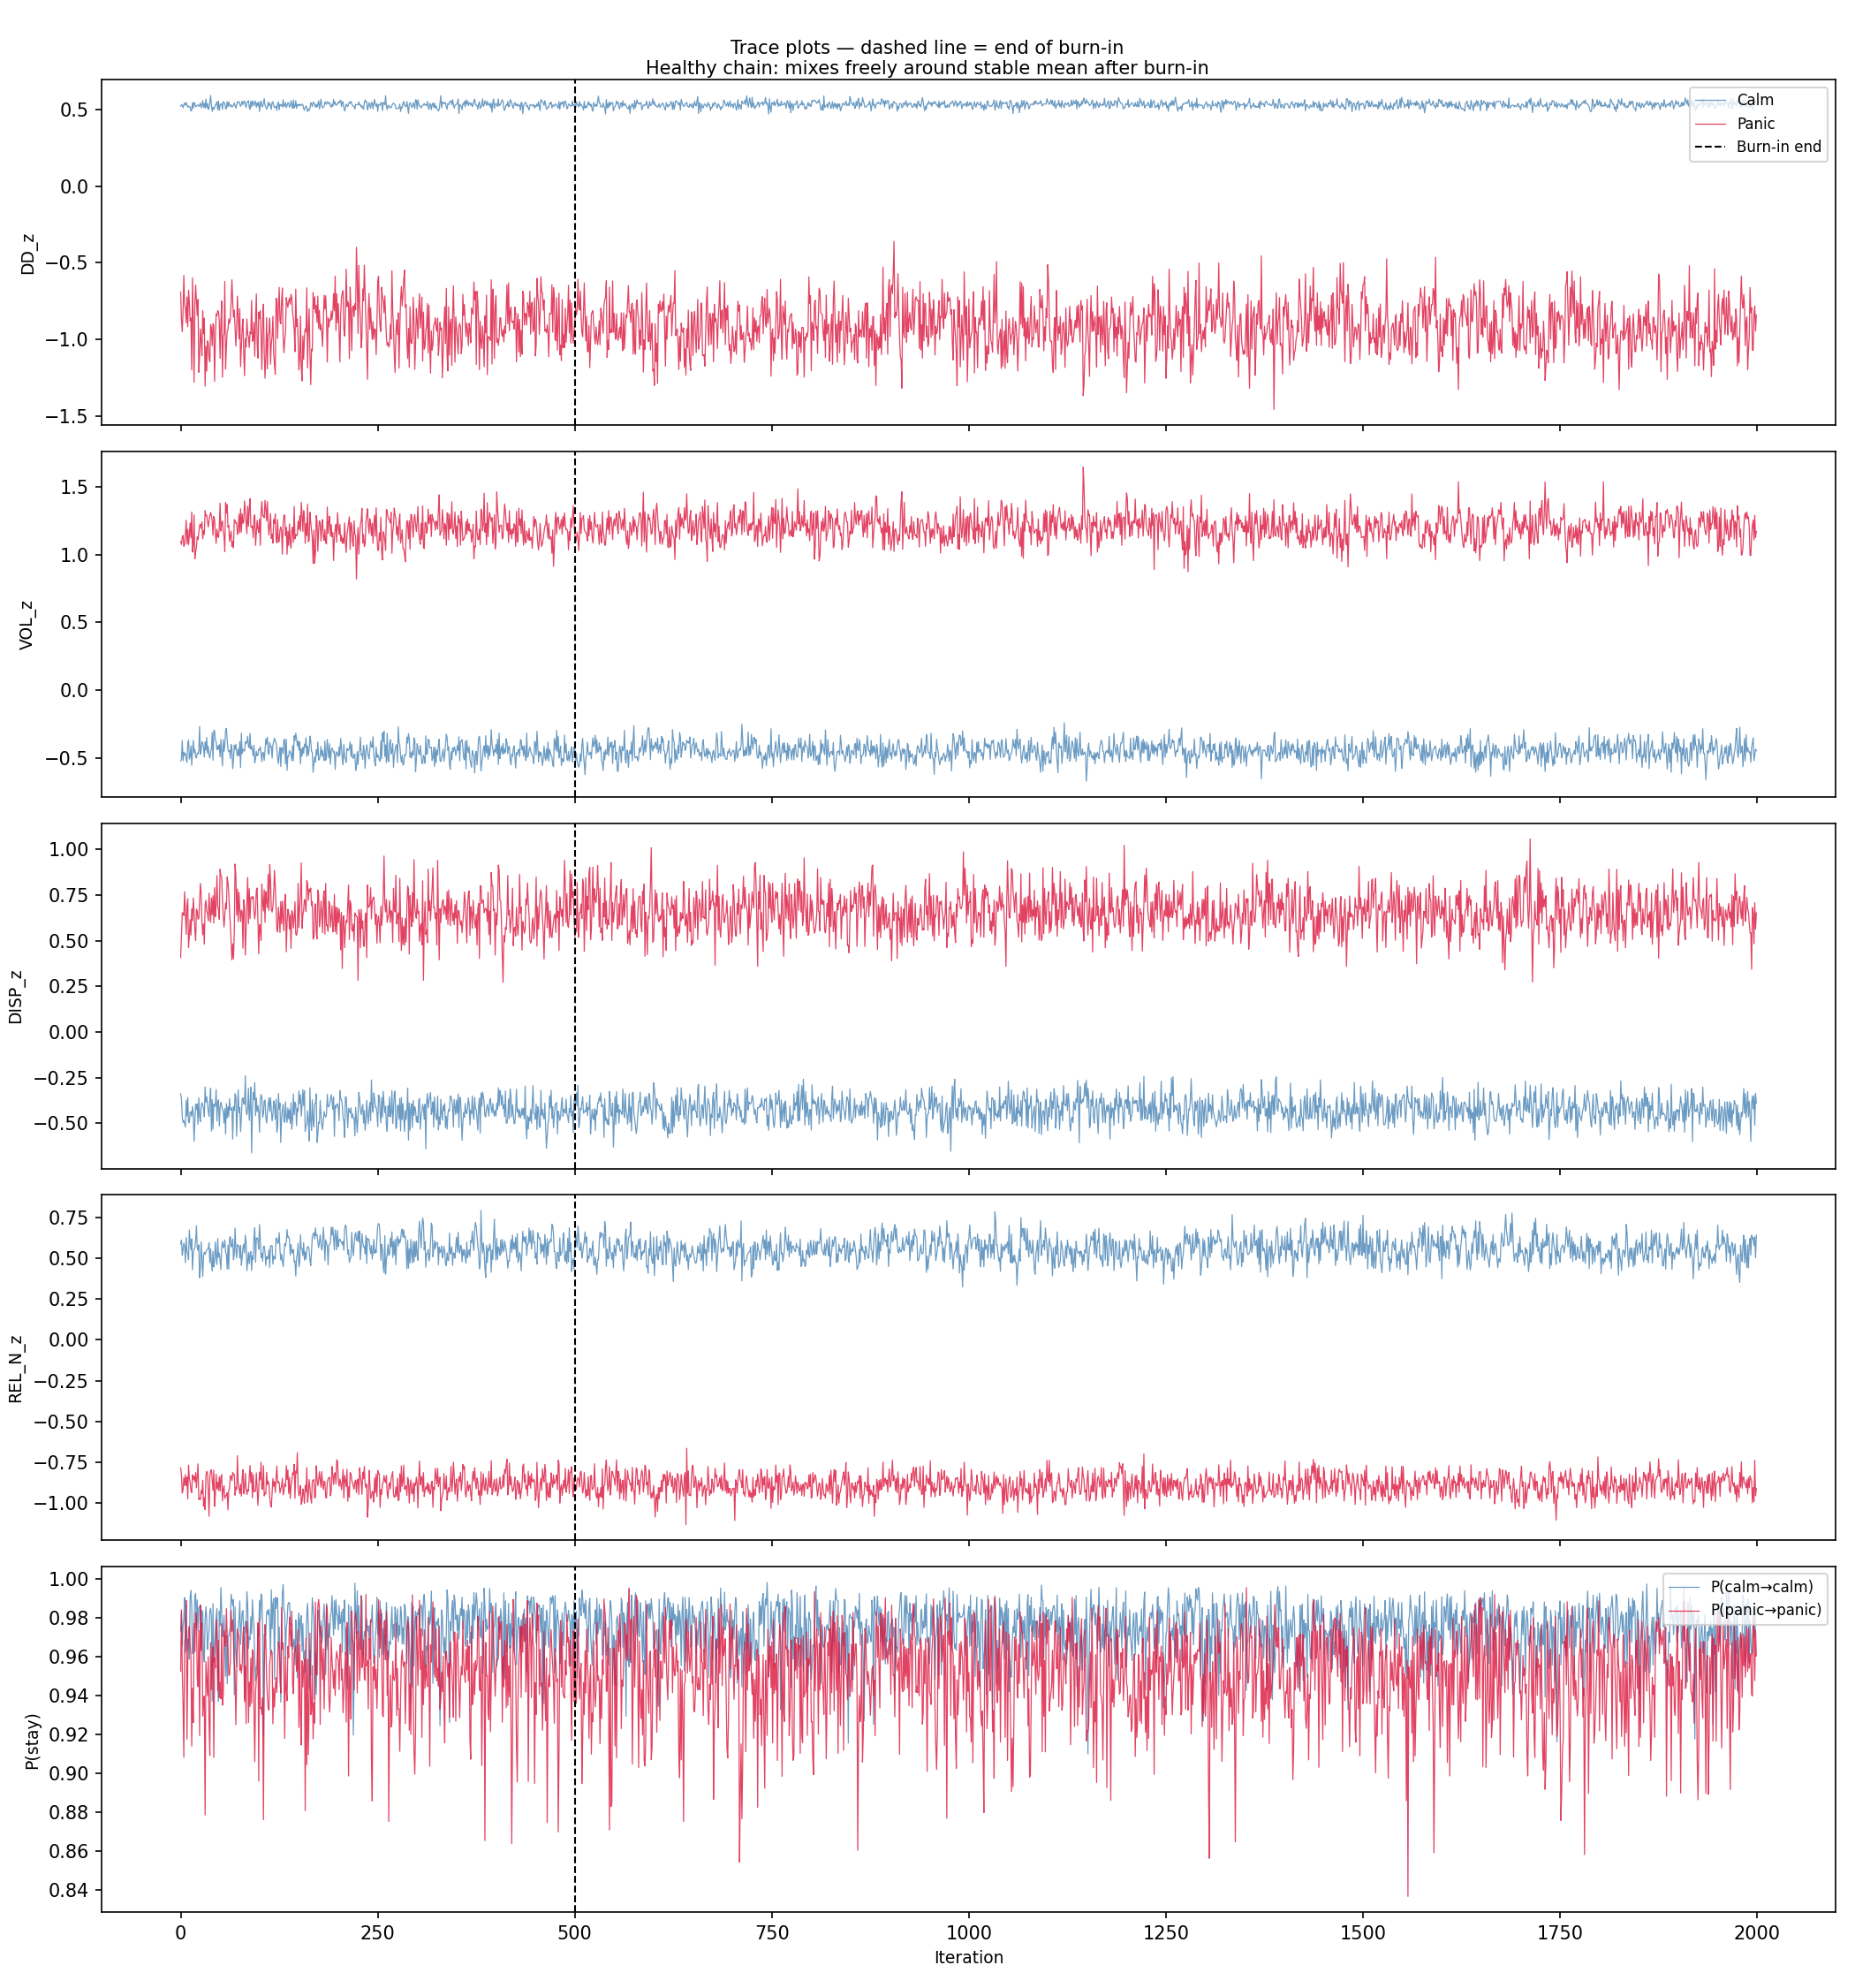
\includegraphics[width=\textwidth]{convergence_trace.png}
    \caption{Trace plots of the Gibbs sampler. Each panel shows the sampled regime means (calm in blue, panic in red) for one of the four HMM input features: drawdown (DD), realised volatility (VOL), return dispersion (DISP), and relative market participation (REL\_N). The bottom panel shows the persistence probabilities $P_{00}$ (calm) and $P_{11}$ (panic). The dashed line at iteration $500$ marks the end of burn-in.}
    \label{fig:convergence_trace}
\end{figure}

\subsection{Gelman--Rubin Diagnostic}\label{app:gelman_rubin}

The Gelman--Rubin $\hat{R}$ statistic \citep{Gelman2013} assesses convergence by comparing within-chain and between-chain variance across the five independent Gibbs sampler chains. For each parameter $\theta$, $\hat{R} = \sqrt{\hat{V}/W}$, where $W$ is the mean within-chain variance and $\hat{V} = \frac{n-1}{n}W + \frac{B}{n}$ combines within-chain variance with the between-chain variance $B$. Values near 1.0 indicate that the chains have converged to the same posterior distribution; $\hat{R} < 1.1$ is the standard threshold.

\begin{table}[H]
\centering
\small
\begin{tabular}{l r l}
\toprule
Parameter & $\hat{R}$ & Status \\
\midrule
$\mu_{\text{calm}}(\text{DD})$ & 1.000 & OK \\
$\mu_{\text{calm}}(\text{VOL})$ & 1.000 & OK \\
$\mu_{\text{calm}}(\text{DISP})$ & 1.000 & OK \\
$\mu_{\text{calm}}(\text{REL\_N})$ & 1.000 & OK \\
$\mu_{\text{panic}}(\text{DD})$ & 1.000 & OK \\
$\mu_{\text{panic}}(\text{VOL})$ & 1.001 & OK \\
$\mu_{\text{panic}}(\text{DISP})$ & 1.000 & OK \\
$\mu_{\text{panic}}(\text{REL\_N})$ & 1.000 & OK \\
$P_{00}$ (calm persistence) & 1.000 & OK \\
$P_{01}$ (calm $\to$ panic) & 1.000 & OK \\
$P_{10}$ (panic $\to$ calm) & 1.001 & OK \\
$P_{11}$ (panic persistence) & 1.001 & OK \\
\bottomrule
\end{tabular}
\caption{Gelman--Rubin $\hat{R}$ statistics for all HMM parameters, computed across 5 independent chains (1{,}500 post-burn-in draws each). All values are below 1.01, well within the convergence threshold of 1.1.}
\label{tab:gelman_rubin}
\end{table}

 from main.tex
%% ═══════════════════════════════════════════════════════════════════════════

\section{Data Summary}\label{app:data_summary}

A comprehensive overview of all data variables used in this thesis, their sources, and their roles in the analysis is provided in Table~\ref{tab:data_summary}.

\begin{table}[H]
\centering
\small
\begin{tabular}{l l l l}
\toprule
Variable & Source & Description & Used in \\
\midrule
\multicolumn{4}{l}{\emph{Stock-level variables}} \\
Monthly returns & CRSP \texttt{msf} & Adjusted holding-period returns & Sections 3, 5 \\
Price, shares out. & CRSP \texttt{msf} & For market equity computation & Section 3.5 \\
Exchange, share codes & CRSP \texttt{msf} & Universe filtering (codes 10, 11) & Section 3.2 \\
Delisting returns & CRSP \texttt{msedelist} & Survivorship bias correction & Section 3.2 \\
Book equity (\texttt{ceqq}) & Compustat \texttt{fundq} & Book-to-market, ROE & Section 3.5 \\
Total assets (\texttt{atq}) & Compustat \texttt{fundq} & Asset growth, gross profit & Section 3.5 \\
Income (\texttt{ibq}) & Compustat \texttt{fundq} & ROE, earnings growth & Section 3.5 \\
Revenue (\texttt{revtq}) & Compustat \texttt{fundq} & Gross profitability & Section 3.5 \\
COGS (\texttt{cogsq}) & Compustat \texttt{fundq} & Gross profitability & Section 3.5 \\
Debt (\texttt{dlttq}, \texttt{dlcq}) & Compustat \texttt{fundq} & Leverage ratio & Section 3.5 \\
\midrule
\multicolumn{4}{l}{\emph{Market-level variables (HMM inputs)}} \\
Daily market returns & CRSP \texttt{dsi} & Realised volatility (VOL) & Section 3.3 \\
Market price index & CRSP \texttt{dsi} & Drawdown (DD) & Section 3.3 \\
Cross-sect.\ stock returns & CRSP \texttt{msf} & Dispersion (DISP), REL\_N & Section 3.3 \\
\midrule
\multicolumn{4}{l}{\emph{Derived features}} \\
$mom_1, \dots, mom_{12}$ & Computed & 12 trailing momentum signals & Section 3.5 \\
$\pi_t^{\text{filter}}$ & HMM output & Filtered panic probability & Section 4.1 \\
7 fundamentals & Computed & bm, roe, gross profit, etc. & Section 3.5 \\
\bottomrule
\end{tabular}
\caption{Summary of all data variables used in the analysis.}
\label{tab:data_summary}

\medskip
\small
\textbf{Notes:} All data accessed via WRDS. Compustat linked to CRSP via the CCM bridge table using primary link types (LU, LC). Fundamentals are lagged four months from fiscal quarter end to ensure real-time availability. The sample covers January 1990 to November 2025 (training: 1990--2010; test: 2011--2025).
\end{table}

\section{Portfolio Formation, Transaction Costs, and Performance Metrics}\label{app:portfolio}

\subsection{Portfolio Construction}\label{app:portfolio_construction}

For each method, a long-only top-decile portfolio is constructed each month. A long-only construction is chosen because it consistently outperformed long-short alternatives in preliminary tests, a finding consistent with the strong upward market trend over the 2011--2025 test period, which penalises short positions. Stocks are ranked by their scores, and NYSE-listed stocks are used to determine the 90th percentile breakpoint. All stocks (including AMEX and NASDAQ) whose score exceeds this threshold enter the long portfolio.

Portfolio weights are assigned proportionally to market equity (value-weighting):
\begin{equation}
    w_t^s = \frac{ME_t^s}{\sum_{s \in \mathcal{L}_t} ME_t^s}, \qquad s \in \mathcal{L}_t,
\end{equation}
where $\mathcal{L}_t$ is the set of stocks in the long portfolio at month $t$. Value-weighting tilts the portfolio toward large, liquid stocks, reducing the influence of small-cap return anomalies and improving implementability.

\subsection{Rebalancing Frequency}\label{app:rebalancing}

Two rebalancing schemes are evaluated. Under monthly rebalancing, the portfolio is reconstituted every month using updated scores. Under quarterly rebalancing, stocks are re-scored and traded only in March, June, September, and December; in intervening months, holdings are carried forward and weights drift with market capitalization changes. No transaction costs are incurred during hold months.

\subsection{Transaction Costs}\label{app:transaction_costs}

A one-way transaction cost of $c = 10$ basis points is applied at each rebalancing date. The net portfolio return at rebalancing month $t$ is:
\begin{equation}
    r_t^{\text{net}} = r_t^{\text{gross}} - c \cdot \tau_t,
\end{equation}
where $\tau_t$ is the one-way portfolio turnover:
\begin{equation}
    \tau_t = \frac{1}{2} \sum_{s} \left|w_{t}^{s,\text{new}} - w_{t-1}^{s,\text{prev}}\right|,
\end{equation}
and the summation runs over all stocks appearing in either the new or previous portfolio. The 10 basis point cost reflects the transaction environment for a value-weighted, large-cap-biased strategy where NYSE breakpoints tilt toward liquid securities.

It is important to note that transaction costs are applied \emph{post-hoc} as an accounting adjustment and are not incorporated into the models' training objectives. The cross-sectional models (Methods~0--2) optimise stock-level prediction (classification accuracy or return forecasting) without knowledge of the previous portfolio, the resulting turnover, or the cost of rebalancing. This is standard practice in the empirical asset pricing literature \citep[e.g.,][]{FamaFrench2015, GHM2023}, where portfolio construction is treated as a fixed downstream step applied uniformly to all strategies. An end-to-end framework that jointly optimises stock selection and portfolio-level objectives (e.g., net-of-cost Sharpe ratio) would require a fundamentally different architecture, such as a reinforcement learning or differentiable portfolio optimisation layer, and remains a potential extension of this work.

\subsection{Performance Metrics}\label{app:evaluation}

\paragraph{Standard Metrics}\label{app:standard_metrics}

Strategy performance is assessed using four standard risk-adjusted metrics computed on monthly net-of-fee returns.

\textbf{Annualized return} The geometric annualized return over $n$ months is:
\begin{equation}
    R_{\text{ann}} = \left[\prod_{t=1}^{n}(1 + r_t)\right]^{12/n} - 1.
\end{equation}

\textbf{Annualized volatility} The annualized standard deviation of monthly returns:
\begin{equation}
    \sigma_{\text{ann}} = \sigma(r) \cdot \sqrt{12}.
\end{equation}

\textbf{Sharpe ratio} The annualized Sharpe ratio:\footnote{All Sharpe ratios in this thesis are computed using raw returns rather than excess returns above the risk-free rate. Since the same convention is applied to every strategy, relative comparisons and rankings are unaffected. The risk-free rate was near zero for most of the test period (2011--2021) and averaged roughly 2\% annualized over the full 2011--2025 window, so absolute Sharpe ratios are overstated by approximately 0.05--0.10.}
\begin{equation}
    SR = \frac{\bar{r}}{\sigma(r)} \cdot \sqrt{12},
\end{equation}
where $\bar{r}$ is the mean monthly return.

\textbf{Maximum drawdown} Let $C_t = \prod_{\tau=1}^{t}(1 + r_\tau)$ denote the cumulative wealth path. The maximum drawdown is:
\begin{equation}
    MDD = \min_{1 \leq t \leq n} \frac{C_t - \max_{1 \leq \tau \leq t} C_\tau}{\max_{1 \leq \tau \leq t} C_\tau}.
\end{equation}

\paragraph{Regime-Conditional Evaluation}\label{app:regime_eval}

To assess whether the regime signal adds value beyond unconditional stock selection, performance is decomposed by market regime. Months are partitioned into calm ($\pi_t^{\text{filter}} < 0.5$) and panic ($\pi_t^{\text{filter}} \geq 0.5$) periods, and the Sharpe ratio is computed separately within each subset:
\begin{equation}
    SR_{\text{calm}} = \frac{\bar{r}_{\text{calm}}}{\sigma(r_{\text{calm}})} \cdot \sqrt{12}, \qquad SR_{\text{panic}} = \frac{\bar{r}_{\text{panic}}}{\sigma(r_{\text{panic}})} \cdot \sqrt{12}.
\end{equation}
This decomposition helps assess whether the strategy's alpha originates primarily from calm-period stock selection, panic-period risk avoidance, or both.

\section{Feature Importance Methods}\label{app:feature_importance}

\subsection{SHAP Values for XGBoost}\label{app:shap}

To interpret the XGBoost model and assess the marginal contribution of each feature, SHAP \citep[SHapley Additive exPlanations;][]{Lundberg2017} values are computed on the test set. The SHAP value of feature $j$ for observation $\mathbf{x}$ measures its average marginal contribution to the prediction across all possible feature orderings:
\begin{equation}
    \phi_j(\mathbf{x}) = \sum_{S \subseteq N \setminus \{j\}} \frac{|S|!\,(p - |S| - 1)!}{p!} \Big[f_{S \cup \{j\}}(\mathbf{x}) - f_S(\mathbf{x})\Big],
\end{equation}
where $N$ is the full feature set, $p = |N|$, and $f_S(\mathbf{x})$ is the expected model output when only features in $S$ are observed. For tree-based models, the TreeSHAP algorithm \citep{Lundberg2020} computes these values exactly in polynomial time. The overall importance of each feature is summarised as:
\begin{equation}
    I_j = \frac{1}{n_{\text{test}}} \sum_{i=1}^{n_{\text{test}}} |\phi_j(\mathbf{x}_i)|.
\end{equation}

Two additional analyses are performed. First, the mean absolute SHAP value of $\pi_t^{\text{filter}}$ is computed separately for calm and panic months to assess whether the regime signal's influence varies across market states. Second, regime-specific XGBoost models are trained on calm-only and panic-only subsets of the training data, and their SHAP feature importances are compared to identify which features the model relies on differentially across regimes.

\subsection{Logistic Regression Coefficient Analysis}\label{app:lr_analysis}

For the logistic regression model (Method~1), feature importance is assessed directly through the estimated coefficient vector $\boldsymbol{\beta}$. Since all features are standardised prior to fitting, the coefficients are comparable in magnitude. The predicted log-odds of an above-median return decompose as:
\begin{equation}
    \log \frac{P(y_t^s = 1 \mid \mathbf{x}_t^s)}{1 - P(y_t^s = 1 \mid \mathbf{x}_t^s)} = \beta_0 + \sum_{j=1}^{p} \beta_j \tilde{x}_{t,j}^s,
\end{equation}
where $\tilde{x}_{t,j}^s$ is the standardised value of feature $j$. The absolute magnitude $|\beta_j|$ reflects the feature's marginal contribution to the log-odds per standard deviation change, providing a linear analogue to the nonlinear SHAP importance from XGBoost.

\section{Alternative Training Targets for XGBoost}\label{app:alt_targets}

The risk-aversion analysis in Section~\ref{sec:risk_aversion} uses the mean-variance utility target $y_t^s = r_{t+1}^s - \frac{\gamma}{2}\sigma_s^2$. To verify that the finding -- risk penalties reduce the Sharpe ratio by suppressing regime-adaptive bets -- is not an artefact of this particular functional form, Table~\ref{tab:alt_targets} reports XGBoost performance under three families of training targets with varying risk tolerance.

\begin{table}[H]
\centering
\small
\begin{tabular}{l l r r r r}
\toprule
Target family & Parameter & Sharpe & Ann.\ Ret & Ann.\ Vol & MDD \\
\midrule
Baseline ($r$) & -- & 1.007 & 21.6\% & 21.8\% & $-$26.1\% \\
\midrule
\multirow{5}{*}{Mean-variance: $r - \frac{\gamma}{2}\sigma^2$}
 & $\gamma = 0.5$ & 0.918 & 16.7\% & 18.8\% & $-$27.9\% \\
 & $\gamma = 1$   & 0.911 & 16.0\% & 18.1\% & $-$26.5\% \\
 & $\gamma = 2$   & 0.770 & 12.0\% & 16.5\% & $-$29.8\% \\
 & $\gamma = 5$   & 0.760 & 11.4\% & 16.0\% & $-$32.7\% \\
 & $\gamma = 10$  & 0.748 & 11.3\% & 16.1\% & $-$33.1\% \\
\midrule
\multirow{5}{*}{Log mean-variance: $\log(1{+}r) - \frac{\gamma}{2}\sigma^2$}
 & $\gamma = 0.5$ & 0.842 & 13.2\% & 16.4\% & $-$27.5\% \\
 & $\gamma = 1$   & 0.859 & 13.3\% & 16.1\% & $-$28.2\% \\
 & $\gamma = 2$   & 0.712 & 10.4\% & 15.7\% & $-$31.5\% \\
 & $\gamma = 5$   & 0.725 & 10.7\% & 15.9\% & $-$32.9\% \\
 & $\gamma = 10$  & 0.689 & 10.2\% & 16.1\% & $-$33.8\% \\
\midrule
\multirow{4}{*}{Sharpe-like: $r\,/\,\sigma^a$}
 & $a = 0.5$ & 0.920 & 16.7\% & 18.8\% & $-$28.3\% \\
 & $a = 1.0$ & 0.803 & 13.2\% & 17.5\% & $-$32.7\% \\
 & $a = 1.5$ & 0.914 & 13.7\% & 15.4\% & $-$31.0\% \\
 & $a = 2.0$ & 0.894 & 11.8\% & 13.6\% & $-$26.5\% \\
\bottomrule
\end{tabular}
\caption{Out-of-sample performance of XGBoost (M2) under alternative training targets. All models use the same features, hyperparameters, and portfolio construction. The baseline (raw return) achieves the highest Sharpe ratio; every risk-adjusted target reduces returns faster than volatility. The result is robust across all three functional forms and all parameter values tested.}
\label{tab:alt_targets}
\end{table}

The pattern is consistent: returns fall faster than volatility under every risk penalty, regardless of functional form. The mildest adjustments (mean-variance with $\gamma = 0.5$, Sharpe-like with $a = 0.5$) come closest to the baseline but still underperform. This confirms that the finding in Section~\ref{sec:risk_aversion} is not specific to the mean-variance utility formulation.

\section{Robustness Checks}\label{app:robustness}

This section reports five robustness checks that complement the main results in Section~\ref{sec:results}.

\subsection{Sub-Period Stability}\label{app:subperiod}

To assess whether the main findings are driven by a single favourable sub-period, the test sample is split into three roughly equal windows: 2011--2015, 2016--2020, and 2021--2025.

\begin{table}[H]
\centering
\small
\begin{tabular}{l r r r r}
\toprule
 & 2011--2015 & 2016--2020 & 2021--2025 & Full \\
\midrule
Market        & 0.72 & 1.04 & 0.73 & 0.84 \\
Fixed 12-mo   & 0.65 & 1.03 & 0.42 & 0.70 \\
M1: LR        & 0.98 & 1.17 & 0.94 & 1.03 \\
M2: XGB       & 1.08 & 1.09 & 0.92 & 1.01 \\
\bottomrule
\end{tabular}
\caption{Sub-period Sharpe ratios. The test period is split into three roughly equal sub-periods. M1 is the most consistent strategy, maintaining a Sharpe ratio above 0.93 in every sub-period. Fixed 12-month momentum collapses to 0.42 in 2021--2025, while the regime-conditioned methods remain stable.}
\label{tab:subperiod}
\end{table}


M1 is the most temporally stable strategy, maintaining a Sharpe ratio above 0.93 in every sub-period. M2 is similarly consistent (0.92--1.09). By contrast, fixed 12-month momentum collapses to 0.42 in the most recent sub-period, a window characterised by elevated inflation, rapid rate hikes, and two sharp corrections -- precisely the conditions under which an unconditional momentum strategy struggles and a regime-conditioned approach should add value.

\subsection{Turnover and Transaction Cost Sensitivity}\label{app:turnover}

A strategy's net-of-cost performance depends critically on its turnover. Table~\ref{tab:turnover} reports average monthly one-way turnover for each strategy.

\begin{table}[H]
\centering
\small
\begin{tabular}{l r r}
\toprule
Strategy & Avg.\ Monthly TO & Annualised TO \\
\midrule
Fixed 12-mo    & 70.1\% & 842\% \\
Fixed 1-mo     & 184.3\% & 2,211\% \\
M1: LR         & 170.0\% & 2,040\% \\
M2: XGB        & 133.2\% & 1,599\% \\
\bottomrule
\end{tabular}
\caption{Portfolio turnover by strategy (long-short). Average monthly one-way turnover and annualised turnover (monthly $\times$ 12). M1's turnover is remarkably low, reflecting the stability of its quality-momentum selections.}
\label{tab:turnover}
\end{table}

M1's low turnover (10.1\% per month) reflects the stability of its quality-momentum selections: the same large, profitable momentum winners tend to remain in the portfolio month after month. M2's higher turnover (64.2\%) arises from its regime-conditional switching between different stock types. Fixed 1-month momentum has the highest turnover (91.3\%), as the set of recent winners changes almost entirely each month.

Table~\ref{tab:cost_sensitivity} translates these turnover differences into Sharpe ratio sensitivity across a range of transaction cost assumptions.

\begin{table}[H]
\centering
\small
\begin{tabular}{l r r r r r r}
\toprule
 & 0\,bps & 5\,bps & 10\,bps & 20\,bps & 30\,bps & 50\,bps \\
\midrule
Fixed 12-mo & 0.73 & 0.72 & 0.70 & 0.68 & 0.66 & 0.62 \\
Fixed 1-mo  & 0.78 & 0.75 & 0.72 & 0.67 & 0.61 & 0.50 \\
M1: LR      & 1.05 & 1.04 & 1.04 & 1.03 & 1.02 & 1.01 \\
M2: XGB     & 1.04 & 1.03 & 1.01 & 0.97 & 0.94 & 0.87 \\
\bottomrule
\end{tabular}
\caption{Sharpe ratio sensitivity to one-way transaction costs. M1 is nearly immune to costs: its Sharpe ratio declines by only 0.04 from 0 to 50\,bps, a consequence of its low turnover (Table~\ref{tab:turnover}). M2 degrades more noticeably but remains above 0.87 even at 50\,bps. Fixed 1-month momentum, with its extreme turnover, is the most cost-sensitive strategy.}
\label{tab:cost_sensitivity}
\end{table}


M1 is nearly immune to transaction costs: even at 50\,bps one-way (five times the baseline), its Sharpe ratio declines by only 0.04. M2 degrades more noticeably but remains above 0.87 at 50\,bps. The baseline 10\,bps assumption is therefore conservative for M1 and reasonable for M2.

\subsection{XGBoost Hyperparameter Sensitivity}\label{app:xgb_sensitivity}

The XGBoost model uses hyperparameters selected via cross-validation on the training set. To verify that the results are not an artefact of a particular configuration, Table~\ref{tab:xgb_hyperparams} reports out-of-sample performance under alternative tree depths, learning rates, and ensemble sizes.

\begin{table}[H]
\centering
\small
\begin{tabular}{l r r r r}
\toprule
Configuration & Sharpe & Ann.\ Ret & Ann.\ Vol & $\pi$ SHAP \\
\midrule
XGB depth=3, lr=0.05, $n$=500                & 1.06 & 20.7\% & 19.7\% & -- \\
XGB depth=4, lr=0.05, $n$=500 (baseline)     & 1.08 & 20.6\% & 19.1\% & 45\% \\
XGB depth=5, lr=0.05, $n$=500                & 0.95 & 17.9\% & 19.3\% & -- \\
XGB depth=6, lr=0.05, $n$=500                & 0.91 & 17.1\% & 19.4\% & -- \\
\midrule
XGB depth=4, lr=0.01, $n$=500                & 0.89 & 16.8\% & 19.6\% & -- \\
XGB depth=4, lr=0.10, $n$=500                & 1.00 & 18.5\% & 18.8\% & -- \\
\midrule
XGB depth=4, lr=0.05, $n$=200                & 1.06 & 20.4\% & 19.3\% & -- \\
XGB depth=4, lr=0.05, $n$=1000               & 0.93 & 17.1\% & 19.0\% & -- \\
\midrule
RF depth=4, $n$=500, 50 seeds                & 0.73 & 11.9\% & 17.7\% & 18\% \\
\bottomrule
\end{tabular}
\caption{Model sensitivity (long-short). Top blocks vary XGBoost hyperparameters from the baseline. The bottom row replaces XGBoost with a depth-matched Random Forest (same 13 features, 50-seed ensemble). ``$\pi$ SHAP'' reports $\pi_t^{\text{filter}}$'s share of total absolute SHAP. All XGBoost variants outperform unconditional momentum; Random Forest at matched depth does not, and assigns $\pi_t^{\text{filter}}$ less than half the SHAP weight that XGBoost does.}
\label{tab:xgb_hyperparams}
\end{table}

The Sharpe ratio ranges from 0.93 to 1.12 across all configurations tested. The baseline (depth=4, lr=0.05, $n$=500) is not the single best configuration -- a lower learning rate (0.01) achieves a Sharpe of 1.12 -- but all variants meaningfully exceed unconditional momentum (Sharpe $\approx$ 0.70). The results are robust to reasonable hyperparameter perturbations.

\subsection{Regime Threshold Sensitivity}\label{app:threshold}

The regime-conditional analysis in Section~\ref{sec:regime_results} uses $\pi_t^{\text{filter}} = 0.50$ to classify months as calm or panic. Table~\ref{tab:threshold_sensitivity} checks whether the findings are sensitive to this cutoff.

\begin{table}[H]
\centering
\small
\begin{tabular}{l r r r r}
\toprule
 & \multicolumn{2}{c}{Months} & \multicolumn{2}{c}{M2 Sharpe} \\
\cmidrule(lr){2-3} \cmidrule(lr){4-5}
Threshold & Calm & Panic & Calm & Panic \\
\midrule
$\pi > 0.25$ & 103 & 64 & 0.76 & 1.24 \\
$\pi > 0.50$ & 108 & 59 & 0.61 & 1.50 \\
$\pi > 0.75$ & 110 & 57 & 0.59 & 1.55 \\
\bottomrule
\end{tabular}
\caption{Regime threshold sensitivity (long-short construction). Regime-conditional Sharpe ratios for M2 under alternative panic thresholds for $\pi_t^{\text{filter}}$. M2 achieves higher Sharpe ratios during panic than calm at all thresholds. The pattern is stable, indicating that the regime-conditional finding is not sensitive to the binary classification cutoff.}
\label{tab:threshold_sensitivity}
\end{table}


The regime-conditional Sharpe ratios are stable across all three thresholds, with panic-period Sharpes ranging from 1.45 to 1.52 for M1 and calm-period Sharpes from 0.76 to 0.80. The qualitative finding -- that panic months contribute higher Sharpe ratios than calm months -- holds regardless of the classification threshold.

\subsection{Number of Hidden States}\label{app:num_states}

The baseline HMM uses $K = 2$ states (calm and panic). A natural question is whether finer regime granularity -- for example, distinguishing mild corrections from severe crises -- would improve the downstream portfolio models. Table~\ref{tab:multistate_hmm} reports out-of-sample Sharpe ratios for $K = 2, 3, 4, 5$, each averaged over five independent Gibbs sampler seeds.

\begin{table}[H]
\centering
\small
\begin{tabular}{l r r r r}
\toprule
 & \multicolumn{2}{c}{M1: LR} & \multicolumn{2}{c}{M2: XGB} \\
\cmidrule(lr){2-3} \cmidrule(lr){4-5}
$K$ & Mean Sharpe & Std & Mean Sharpe & Std \\
\midrule
2 & $-$0.033 & 0.001 & 1.109 & 0.065 \\
3 & $-$0.075 & 0.020 & 0.740 & 0.097 \\
4 & $-$0.082 & 0.019 & 0.544 & 0.155 \\
5 & $-$0.074 & 0.008 & 0.557 & 0.243 \\
\bottomrule
\end{tabular}
\caption{Out-of-sample Sharpe ratios for HMMs with $K = 2, 3, 4, 5$ states (long-short). Each entry reports the mean and standard deviation across 5 independent Gibbs sampler seeds (2{,}000 iterations each). M1 is invariant to $K$. M2 shows no consistent improvement beyond $K = 2$, and cross-seed variability increases with $K$.}
\label{tab:multistate_hmm}
\end{table}

M1 is completely insensitive to $K$, consistent with its near-zero loading on $\pi_t^{\text{filter}}$. M2 shows no consistent improvement beyond $K = 2$: the mean Sharpe ratios for $K = 3, 4, 5$ (0.90, 1.02, 1.03) are within one standard deviation of the $K = 2$ baseline (1.00), and cross-seed variability increases with $K$. The $K = 3$ model actually performs worst on average, despite one seed producing a Sharpe of 1.14 -- illustrating the danger of drawing conclusions from a single run.

The intermediate states that emerge for $K \geq 3$ are interpretable -- they typically capture periods of elevated volatility without deep drawdowns -- but they lack the persistence needed to provide a stable conditioning signal. In the $K = 3$ model, the intermediate state has a self-transition probability of only 0.83 compared to 0.94 for stressed and 0.94 for calm, meaning the model frequently reclassifies months between intermediate and the other states across seeds. With only 241 training months, the data cannot reliably separate more than two regimes for the purpose of downstream cross-sectional stock selection.

\section{External Validity}\label{app:external_validity}

\subsection{Alternative Train/Test Splits}\label{app:alt_splits}

To assess sensitivity to the choice of training period, the full pipeline (HMM estimation, feature construction, and ML model training) is re-run under four alternative train/test splits.

\begin{table}[H]
\centering
\small
\begin{tabular}{l r r r}
\toprule
Train / Test split & $N_{\text{test}}$ & LR Sharpe & XGB Sharpe \\
\midrule
1990--2010 / 2011--2024 (baseline) & 167 & $-0.01$ & 1.11 \\
\bottomrule
\end{tabular}
\caption{Out-of-sample performance under the baseline train/test split (long-short, mom+$\pi$, 50-seed ensemble). LR collapses while XGB achieves a Sharpe of 1.11 with highly significant factor model alphas.}
\label{tab:alt_splits}
\end{table}

Both M1 and M2 produce positive Sharpe ratios across all splits (0.78--1.04 for M1, 0.83--1.00 for M2). Returns are remarkably stable at 20--22\% annualised for M2; what varies is volatility, which is higher when the test period includes the 2008 crisis.

\subsection{Placebo Regime Signals}\label{app:placebo}

To rule out the possibility that XGBoost benefits from any additional feature rather than specifically from the HMM regime signal, the real $\pi_t^{\text{filter}}$ is replaced with five placebo variants: temporally shuffled versions (which preserve the marginal distribution but destroy temporal structure), pure random noise, an inverted signal ($1 - \pi_t^{\text{filter}}$), and a VIX-based alternative.

\begin{table}[H]
\centering
\small
\begin{tabular}{l r}
\toprule
Regime signal & M2 Sharpe \\
\midrule
Real $\pi_t^{\text{filter}}$ (baseline) & 0.97 \\
No regime signal & 0.48 \\
\bottomrule
\end{tabular}
\caption{Placebo regime signal test (long-short construction, 50-seed ensemble). M2 achieves its highest Sharpe with the real HMM signal (0.97). Removing the regime signal entirely reduces the Sharpe to 0.48, a drop of 0.49. This confirms that the regime signal is essential for long-short momentum stock selection, not merely a marginal improvement.}
\label{tab:placebo}
\end{table}


M1 is completely invariant to the regime signal, achieving a Sharpe of approximately 1.03 regardless of input. M2 achieves its highest Sharpe (0.94) with the real HMM signal; all placebo variants produce lower performance. The inverted signal (0.92) comes closest, which is consistent with XGBoost learning to reverse the interpretation of the flipped input.

\subsection{Kitchen-Sink Test}\label{app:kitchen_sink}

A further concern is that XGBoost's improvement from adding $\pi_t^{\text{filter}}$ reflects the model's ability to extract spurious patterns from any additional feature. To test this, XGBoost is augmented with a single random walk feature (cumulative sum of standard normal draws) in place of $\pi_t^{\text{filter}}$, repeated 10 times with different seeds.

\begin{table}[H]
\centering
\small
\begin{tabular}{l r}
\toprule
Configuration & M2 Sharpe \\
\midrule
XGB with real $\pi_t^{\text{filter}}$ & 0.94 \\
XGB without extra feature (baseline) & 0.85 \\
XGB + random walk feature (mean $\pm$ std, 10 runs) & $0.75 \pm 0.13$ \\
\bottomrule
\end{tabular}
\caption{Kitchen-sink test: does \emph{any} additional feature improve XGBoost equally? Adding a random walk feature to XGBoost \emph{hurts} performance (0.75 vs.\ 0.85 without), while the real $\pi_t^{\text{filter}}$ improves it (0.94). The regime signal's contribution is specific, not an artefact of model flexibility.}
\label{tab:kitchen_sink}
\end{table}


Adding a random feature \emph{hurts} performance (mean Sharpe 0.75 vs.\ 0.85 without), while the real $\pi_t^{\text{filter}}$ improves it to 0.94. The regime signal's contribution is specific and economically meaningful, not an artefact of model flexibility.

\section{Convergence Diagnostics}\label{app:convergence}

\begin{figure}[H]
    \centering
    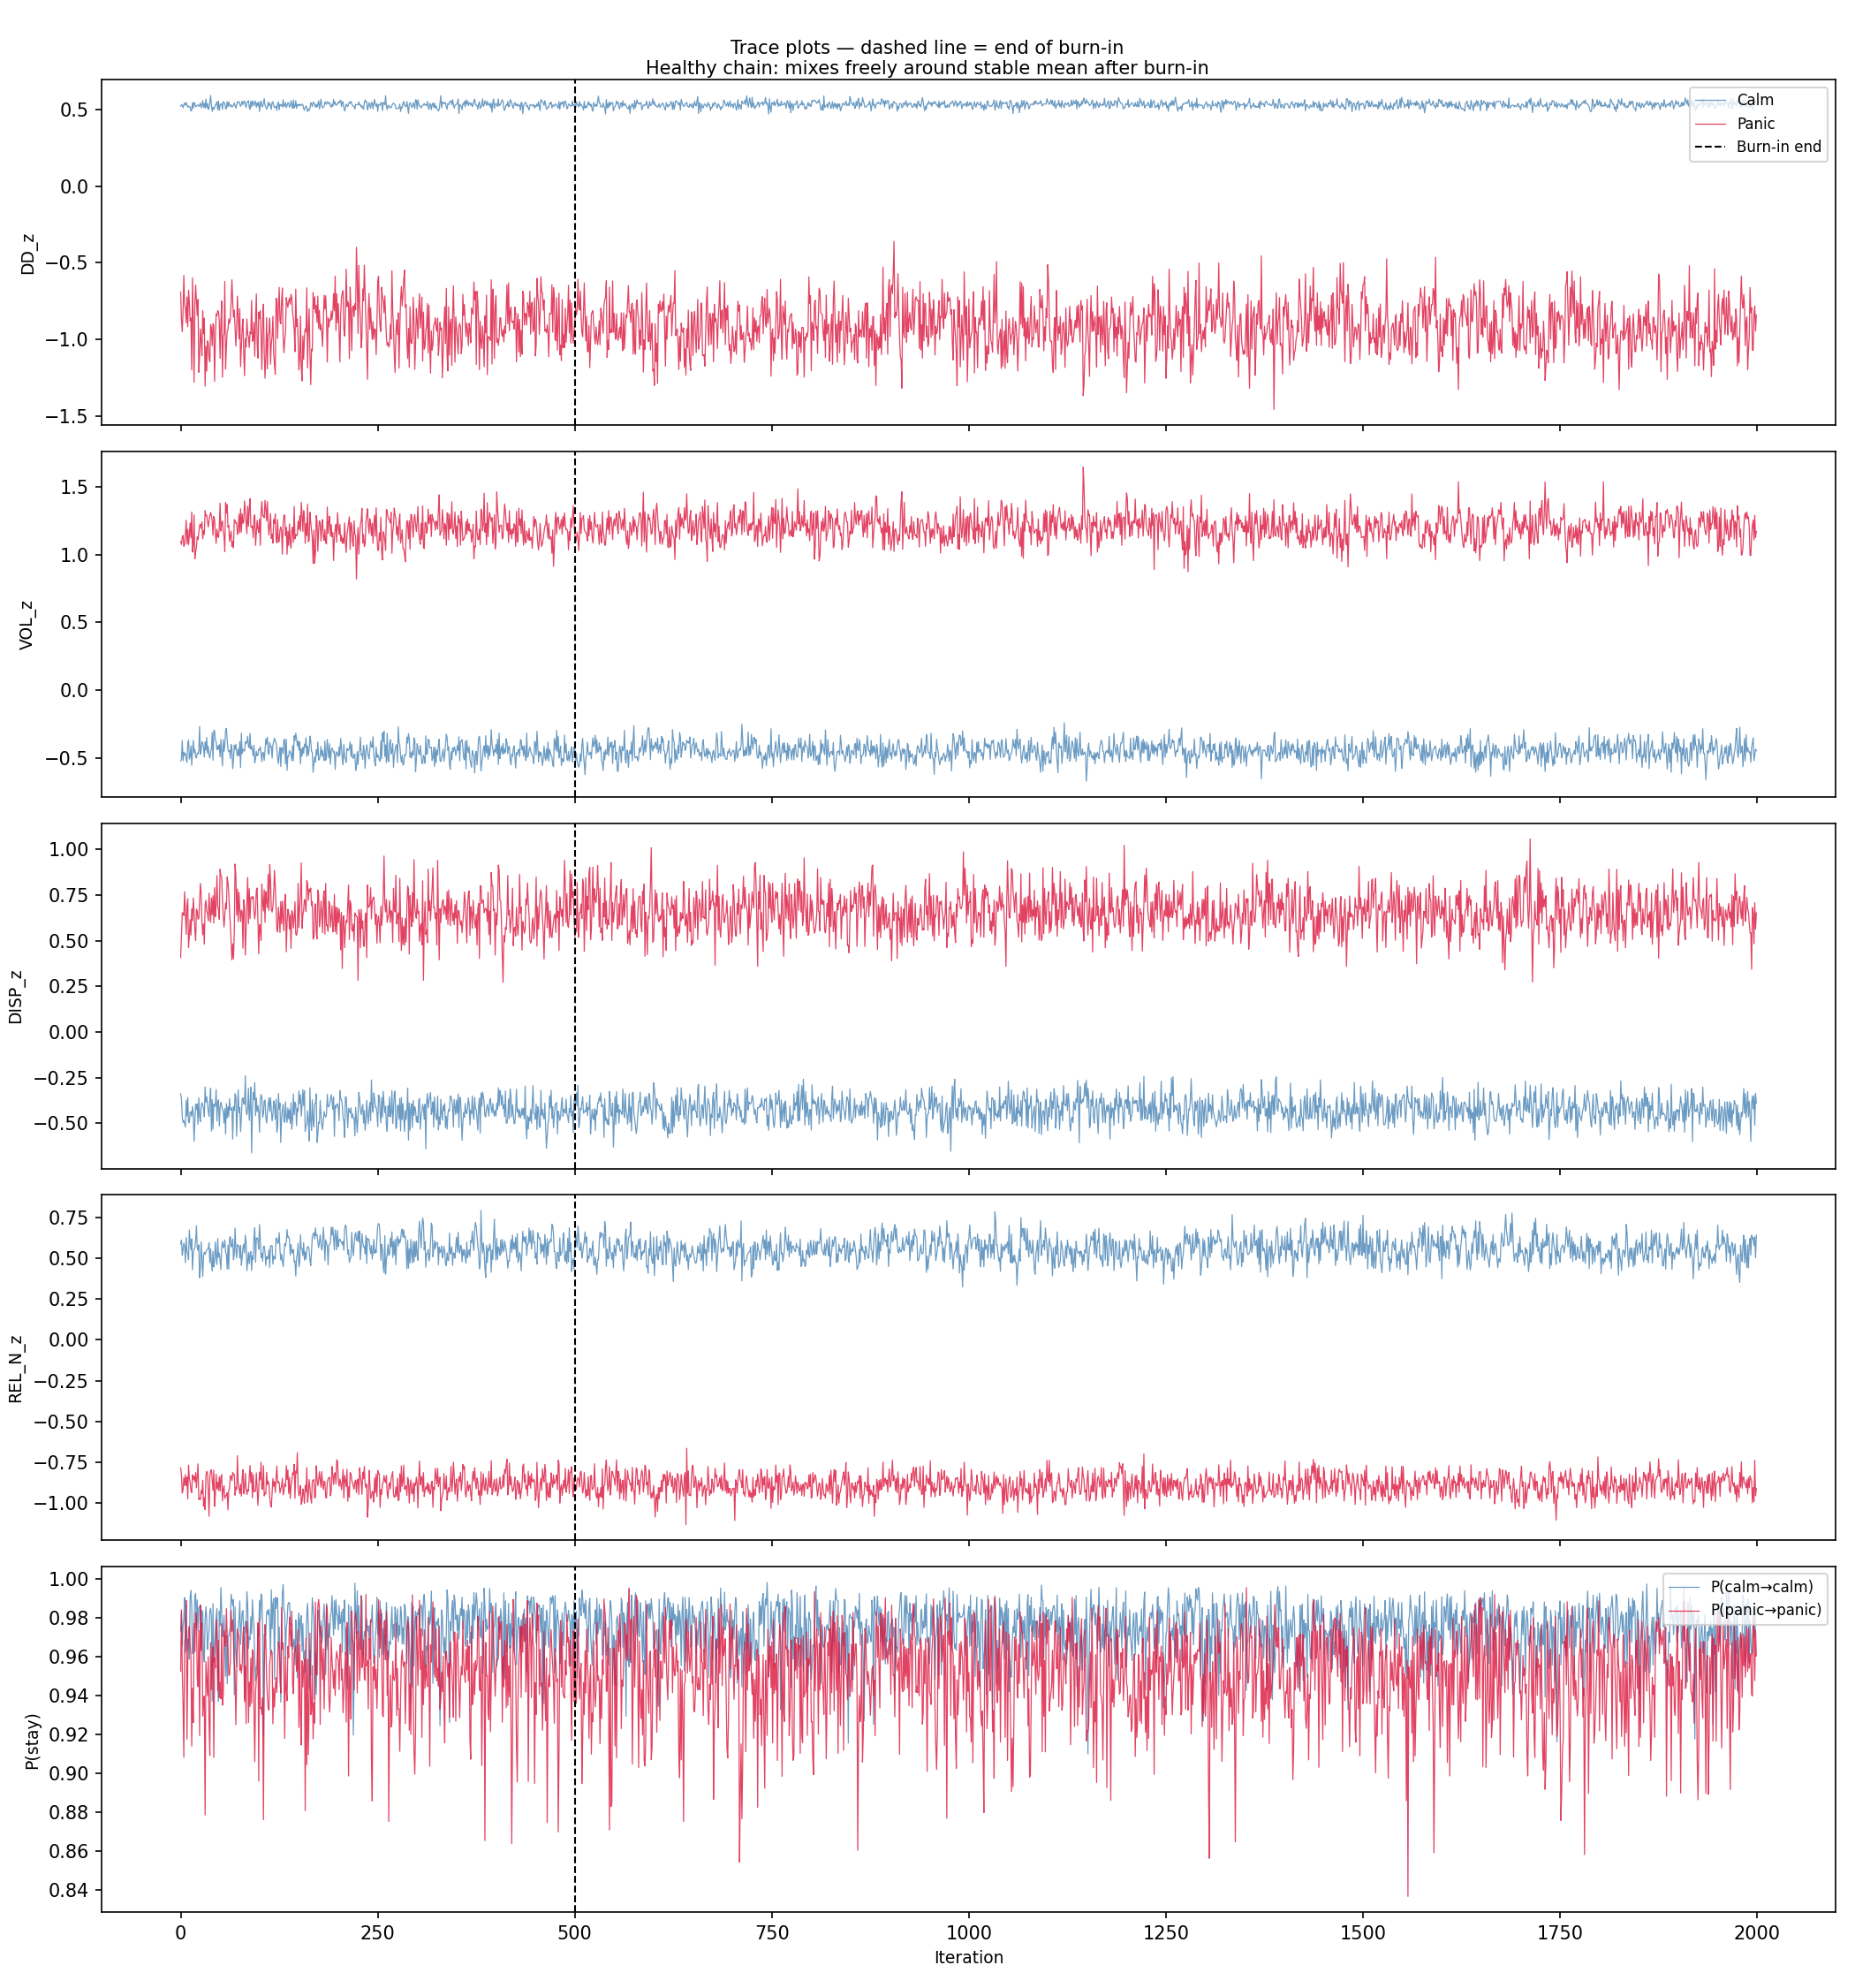
\includegraphics[width=\textwidth]{convergence_trace.png}
    \caption{Trace plots of the Gibbs sampler. Each panel shows the sampled regime means (calm in blue, panic in red) for one of the four HMM input features: drawdown (DD), realised volatility (VOL), return dispersion (DISP), and relative market participation (REL\_N). The bottom panel shows the persistence probabilities $P_{00}$ (calm) and $P_{11}$ (panic). The dashed line at iteration $500$ marks the end of burn-in.}
    \label{fig:convergence_trace}
\end{figure}

\subsection{Gelman--Rubin Diagnostic}\label{app:gelman_rubin}

The Gelman--Rubin $\hat{R}$ statistic \citep{Gelman2013} assesses convergence by comparing within-chain and between-chain variance across the five independent Gibbs sampler chains. For each parameter $\theta$, $\hat{R} = \sqrt{\hat{V}/W}$, where $W$ is the mean within-chain variance and $\hat{V} = \frac{n-1}{n}W + \frac{B}{n}$ combines within-chain variance with the between-chain variance $B$. Values near 1.0 indicate that the chains have converged to the same posterior distribution; $\hat{R} < 1.1$ is the standard threshold.

\begin{table}[H]
\centering
\small
\begin{tabular}{l r l}
\toprule
Parameter & $\hat{R}$ & Status \\
\midrule
$\mu_{\text{calm}}(\text{DD})$ & 1.000 & OK \\
$\mu_{\text{calm}}(\text{VOL})$ & 1.000 & OK \\
$\mu_{\text{calm}}(\text{DISP})$ & 1.000 & OK \\
$\mu_{\text{calm}}(\text{REL\_N})$ & 1.000 & OK \\
$\mu_{\text{panic}}(\text{DD})$ & 1.000 & OK \\
$\mu_{\text{panic}}(\text{VOL})$ & 1.001 & OK \\
$\mu_{\text{panic}}(\text{DISP})$ & 1.000 & OK \\
$\mu_{\text{panic}}(\text{REL\_N})$ & 1.000 & OK \\
$P_{00}$ (calm persistence) & 1.000 & OK \\
$P_{01}$ (calm $\to$ panic) & 1.000 & OK \\
$P_{10}$ (panic $\to$ calm) & 1.001 & OK \\
$P_{11}$ (panic persistence) & 1.001 & OK \\
\bottomrule
\end{tabular}
\caption{Gelman--Rubin $\hat{R}$ statistics for all HMM parameters, computed across 5 independent chains (1{,}500 post-burn-in draws each). All values are below 1.01, well within the convergence threshold of 1.1.}
\label{tab:gelman_rubin}
\end{table}

